\section{Introduction}

In Chapters \ref{sec:chpt_msd}-\ref{sec:chpt_rcca}, we stack observations in a data
matrix that is assumed low-rank plus noise, modeled as
\beq\label{eq:chpt7:data_model}
\widetilde{X}_n= \sum_{i=1}^r\theta_i u_iv_i^T + X_n.
\eeq
In the above equation, for $i=1,\dots,r$, $u_i\in\complex^{n\times 1}$ and
$v_i\in\complex^{N\times 1}$ are independent unit norm signal vectors, $\theta_i>0$ are
the associated signal values and $X_n$ is a noise-only matrix. Assume that
$u_i^Hu_j=\delta_{\left\{i=j\right\}}$ and $v_i^Hv_j = \delta_{\left\{i=j\right\}}$. Let
$X_n\in\complex^{n\times N}$ be a real or complex random matrix. Let 
$\sigma_1,\dots,\sigma_{\min(n,N)}$ be the singular values of $X_n$. Let $\mu_{X_n}$ be the
empirical singular value distribution, i.e, the probability measure defined as
\be
\mu_{X_n} = \frac{1}{\min(n,N)}\sum_{i=1}^{\min(n,N)}\delta_{\sigma_i}.
\ee
Assume that as $n\to\infty$, $n/N\to c_1$. 

In many signal processing applications, we treat the columns of $\widetilde{X}_n$ as noisy
observations of a desired target signal lying in the span of
$\left\{u_1,\dots,u_r\right\}$. In this light, we treat $\theta_i$ as the signal-to-noise
ratio (SNR) for its corresponding subspace component, $n$ as the intrinsic dimension of
the problem, and $N$ as the number of samples (or snapshots or observations) we have at our
disposal. To recover the underlying signal subspace, $\Span\left\{u_1,\dots,u_r\right\}$,
it is common to take the left singular vectors of $\widetilde{X}_n$ corresponding to the
largest $r$ singular values. The accuracy of this estimate is well studied (see
\cite{paul2007asymptotics,benaych2011eigenvalues,asendorf2013performance,benaych2012singular}).
Specifically, when $X_n$ has independent $\mathcal{CN}(0,1)$ entries, the
individual subspace component estimates are known to have a non-random estimate when
$\theta_i>\left(\frac{n}{N}\right)^{1/4}$.

However, in many such applications the intrinsic dimension, $n$, of the system is so large
that taking the SVD of $\widetilde{X}_n$ may not be tractable. In this chapter, we explore the
performance of signal detection when randomly projecting $\widetilde{X}$ into a lower
dimensional space using either a Gaussian or unitary projection. Specifically for $m<n$, let
$G_n\in\complex^{n\times m}$ be a random matrix with independent $\mathcal{CN}(0,1)$
entries and let $Q_n\in\complex^{n\times m}$ be a unitary matrix such that $Q_n^HQ_n=
I_m$. Define the $m\times N$ complex matrices
\beq\label{eq:chpt7:yn}\ba
&Y_n^G = G_n^H\widetilde{X}_n\\
&Y_n^Q = Q_n^H\widetilde{X}_n\\
\ea\eeq

Since $m<n$, taking the SVD of $Y_n^G$ and $Y_n^Q$ is more tractable than taking the SVD
of $\widetilde{X}_n$.  Since $m<n$, taking the SVD of $Y_n^G$ and $Y_n^Q$ is more tractable than taking the SVD
of $\widetilde{X}_n$. Such compressed sensing strategies for both unitary
\cite{belabbas2007fast,gu1996efficient,rudelson2007sampling} and Gaussian
\cite{hehyperspectral,rokhlin2009randomized,halko2011algorithm} sensing matrices have been
extensively studied. These algorithms have been extended to include Gaussian-like
strategies that employ matrices with partially observed entries
\cite{achlioptas2007fast,arora2006fast} as well as unitary-like strategies that use a
discrete Fourier transform matrix \cite{liberty2007randomized} or discrete cosine transform
\cite{ramachandra2011compressive}. For excellent reviews of such compressed sensing
algorithms please see \cite{halko2011finding,candes2006near,donoho2006compressed}, for
example. 

These works examine the ability of such matrices to approximate the original data matrix
as low rank. In this chapter, we consider the fundamental limits of the resulting singular
values when used to detect low-rank signals. We quantify how the dimensions of our
matrices, $m,n,N$, and the SNR $\theta$ affect the behavior of the largest singular values
of $Y_n^G$ and $Y_n^Q$. Finally, we compare the detection performance of these two
specific choices of the projection matrix and show that a unitary projection matrix can
more reliably detect low-rank signals than a Gaussian projection matrix.

Our main conclusion is summarized in Figures \ref{fig:chpt7:motivation1} and
\ref{fig:chpt7:motivation2}. In both figures, we consider a rank-1 setting where $r=1$. In
Figure \ref{fig:chpt7:motivation1}, the SNR of the lone signal is large enough so that the
largest singular value of both $Y_n^G$ and $Y_n^Q$ separate from the bulk of the singular
values. The top singular values of these matrices detect the presence of our lone
signal. In Figure \ref{fig:chpt7:motivation2}, we decrease the SNR of the lone signal. In
this simulation, the largest singular value of $Y_n^Q$ continues to separate from the bulk
distribution but the largest singular value of $Y_n^G$ no longer separates from the bulk
distribution. The unitary projection can reliably detect the presence of signal vectors at
a lower SNR than the Gaussian projection.

This chapter is organized as follows. In Section \ref{sec:chpt7:main_results}, we provide
the main results of this chapter including the almost sure limit of the top singular
values of the projection matrices in (\ref{eq:chpt7:yn}). We then provide corollaries to
the main result that highlight a phase transition below which signal detection is
impossible and a closed form expression of our main theorem for unitary projections. We
provide the proof of our main theorem in Section \ref{sec:chpt7:proof} and the proof of the
main corollary in Section \ref{sec:chpt7:corr_proof}. In Section \ref{sec:chpt7:emp_res},
we verify our asymptotic results on finite sized systems and highlight the accuracy of our
predictions. We make the following assumptions and definitions about the random
matrices needed throughout the rest of the chapter.

\begin{figure}
\begin{center}
  \subfigure[$\widetilde{X}$]{
    \label{fig:chpt7:motiv_full1}
    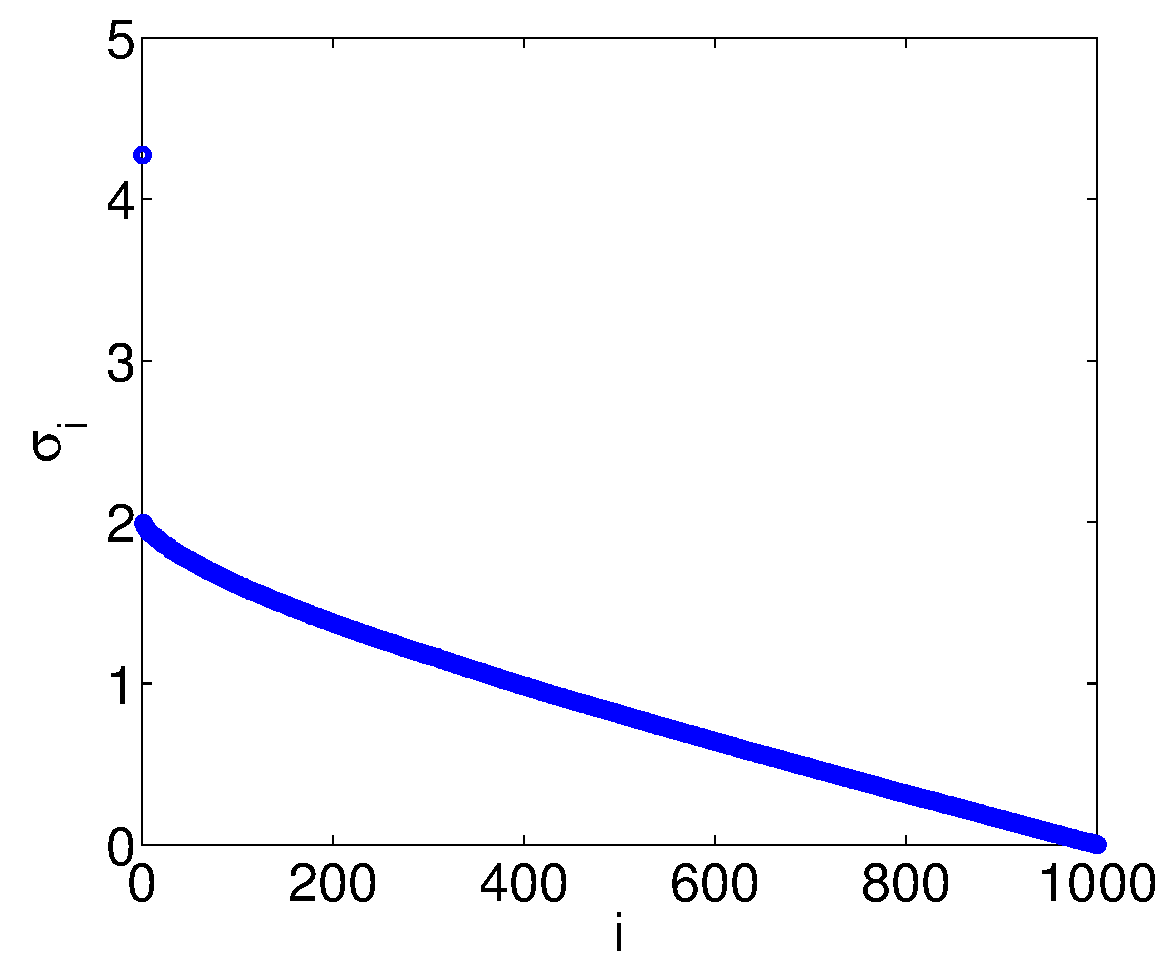
\includegraphics[width=0.3\textwidth]{chpt7_svd_proj/figs/motiv_full_1.pdf}
  }
  \subfigure[$Q^H\widetilde{X}$]{
    \label{fig:chpt7:motiv_orth1}
    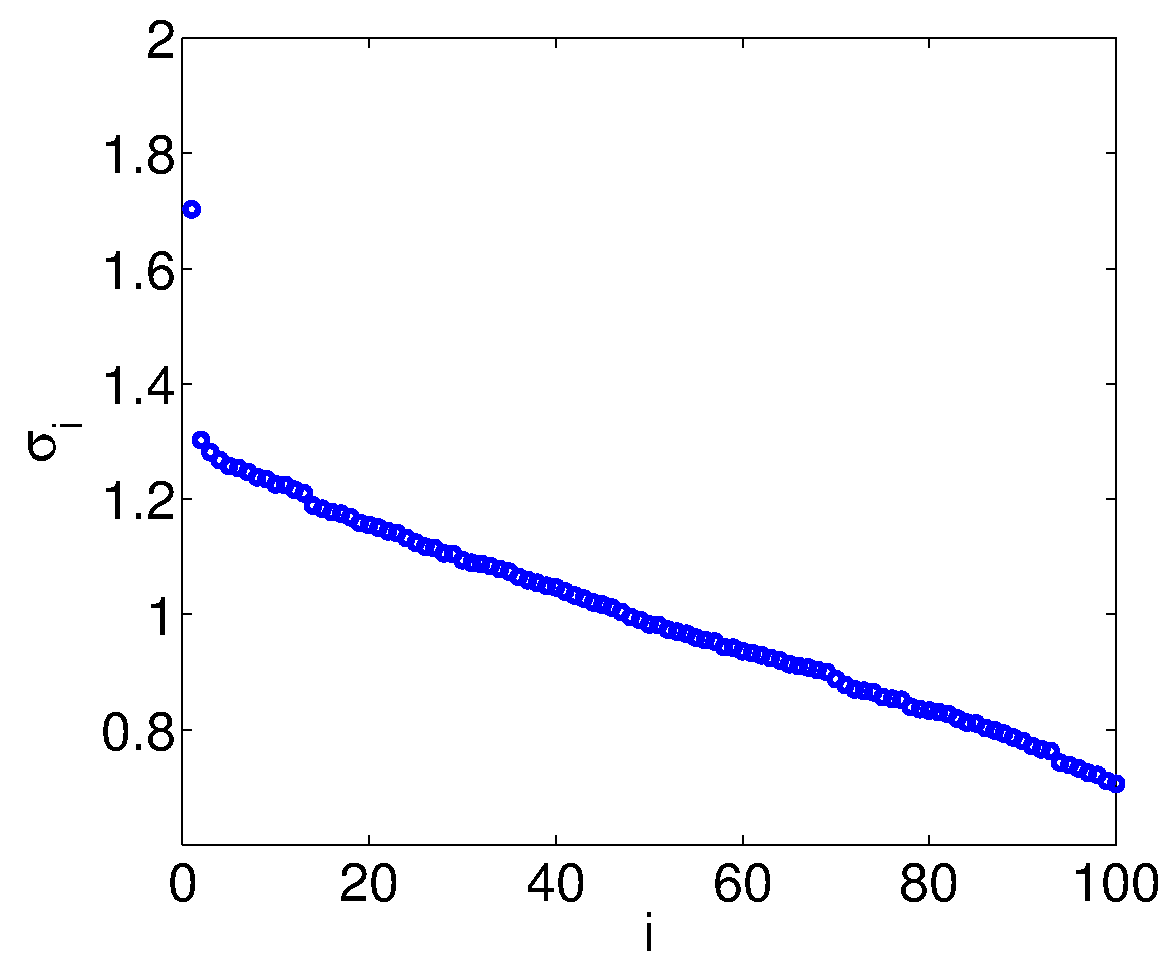
\includegraphics[width=0.3\textwidth]{chpt7_svd_proj/figs/motiv_orth_1.pdf}
  }
  \subfigure[$G^H\widetilde{X}$]{
    \label{fig:chpt7:motiv_gauss1}
   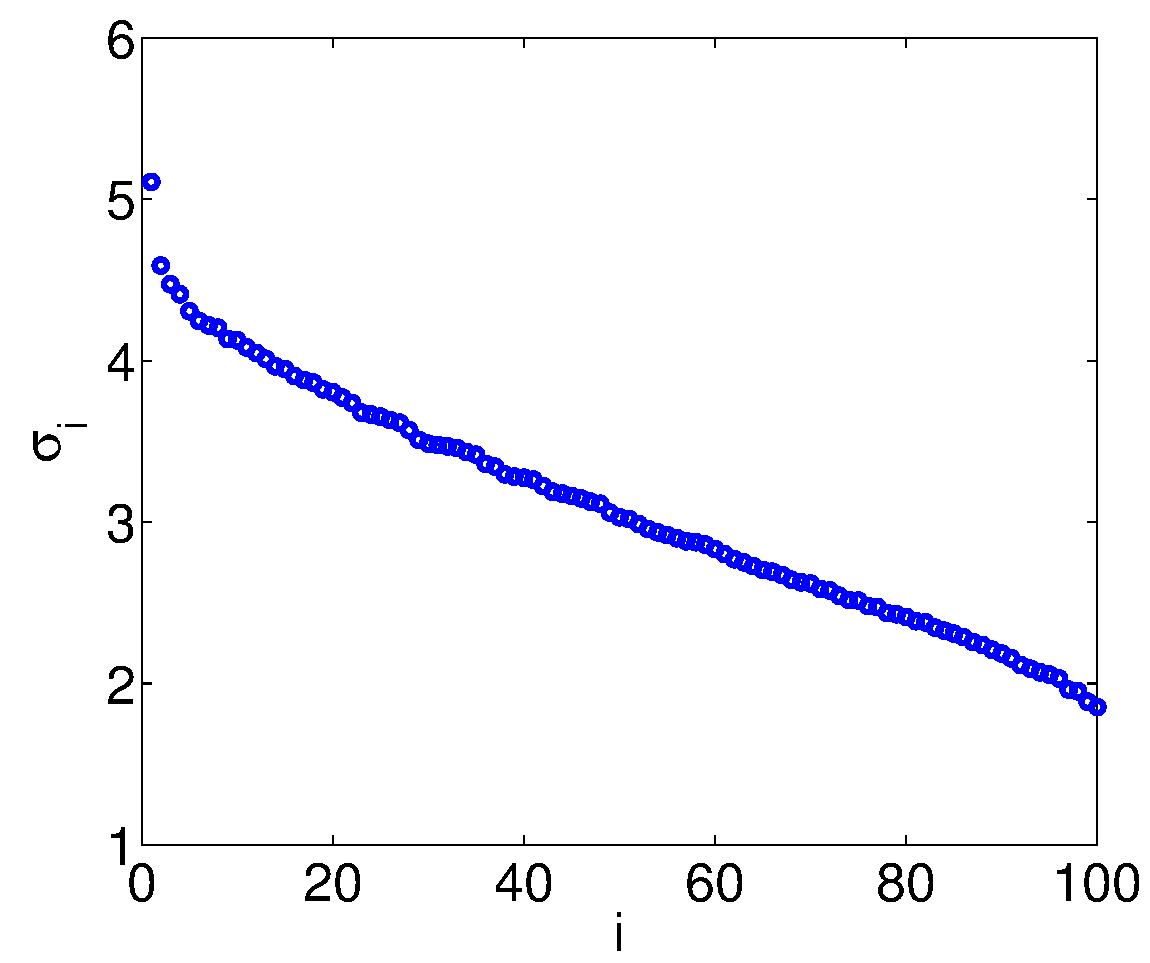
\includegraphics[width=0.3\textwidth]{chpt7_svd_proj/figs/motiv_gauss_1.pdf}
  }
  \caption{Singular value spectra for the full matrix (a), orthogonal projection matrix
    (b), and Gaussian projection matrix (c). This example uses a rank-1
    setting where $n=1000$, $m=100$, $N=1000$, $\theta=\theta_x=\theta_y=4$.}
  \label{fig:chpt7:motivation1}
\end{center}
\end{figure}

\begin{figure}
\begin{center}
  \subfigure[$\widetilde{X}$]{
    \label{fig:chpt7:motiv_full2}
    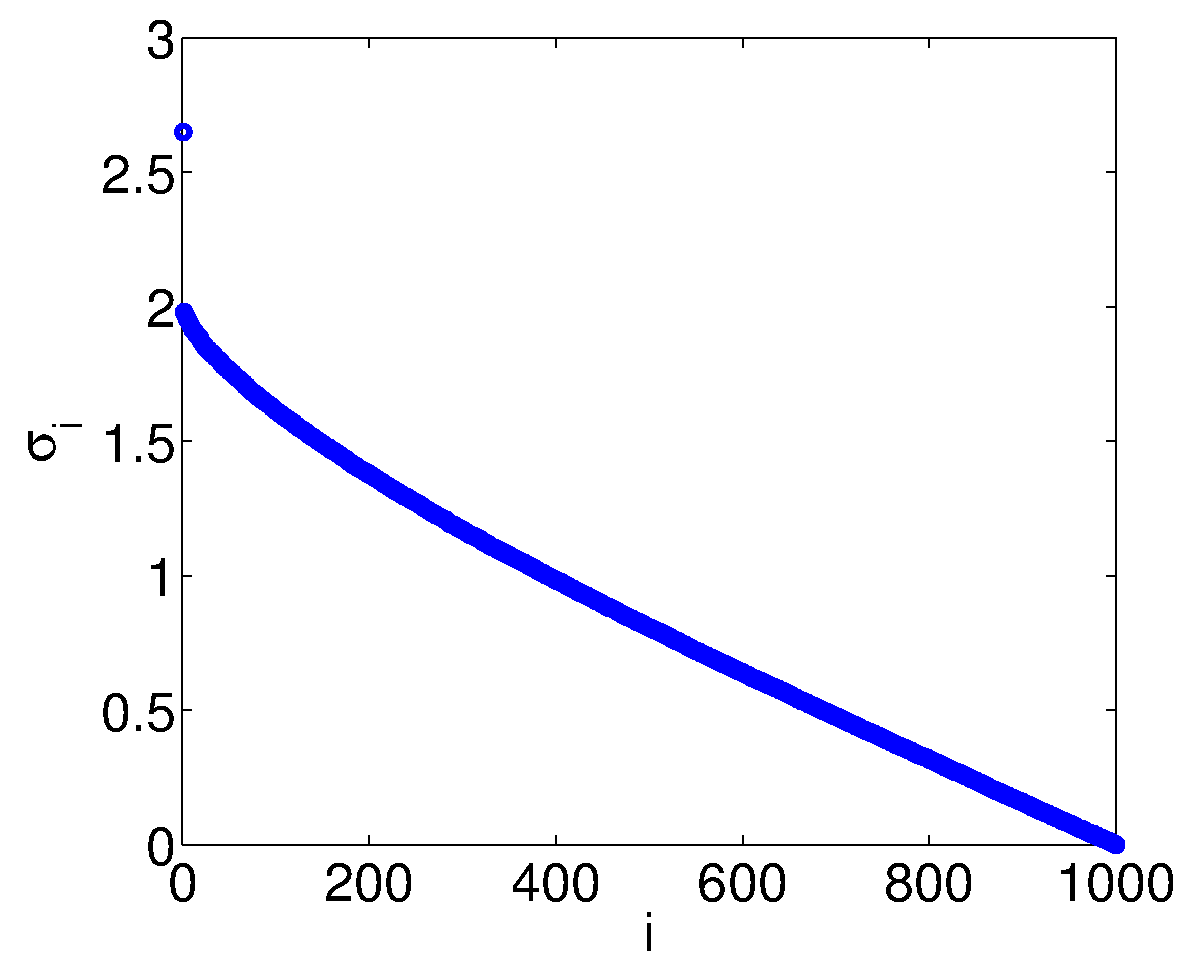
\includegraphics[width=0.3\textwidth]{chpt7_svd_proj/figs/motiv_full_2.pdf}
  }
  \subfigure[$Q^H\widetilde{X}$]{
    \label{fig:chpt7:motiv_orth2}
    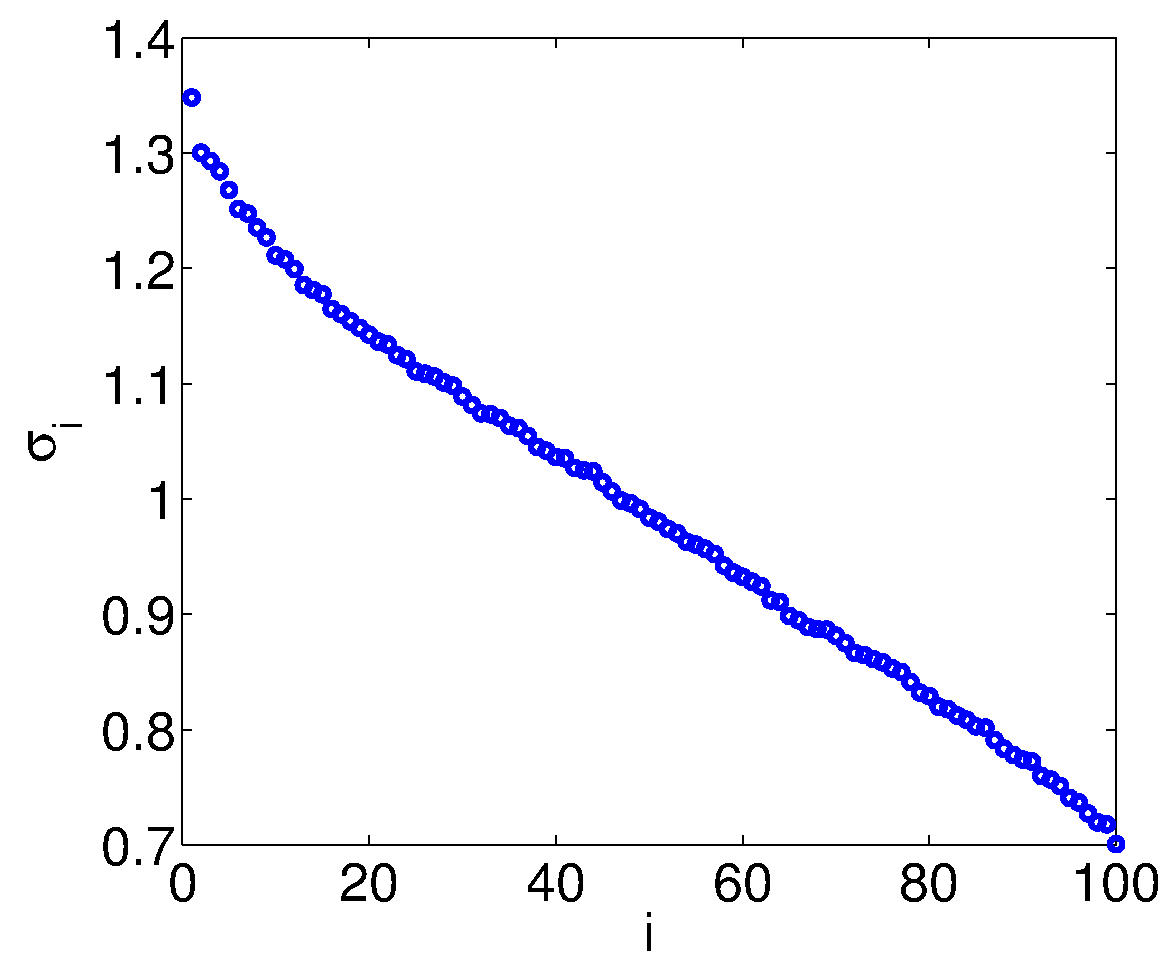
\includegraphics[width=0.3\textwidth]{chpt7_svd_proj/figs/motiv_orth_2.pdf}
  }
  \subfigure[$G^H\widetilde{X}$]{
    \label{fig:chpt7:motiv_gauss2}
   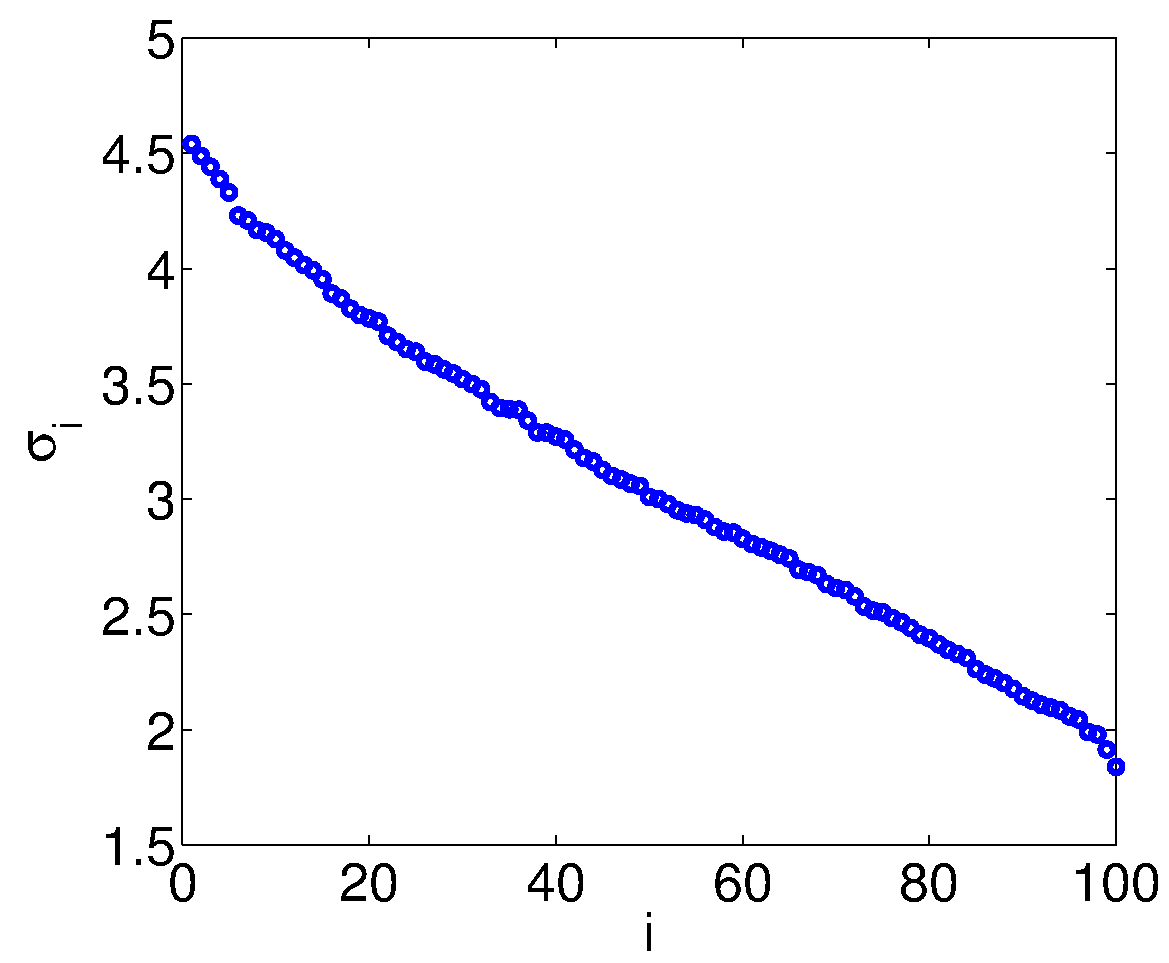
\includegraphics[width=0.3\textwidth]{chpt7_svd_proj/figs/motiv_gauss_2.pdf}
  }
  \caption{Singular value spectra for the full matrix (a), orthogonal projection matrix
    (b), and Gaussian projection matrix (c). This example uses a rank-1
    setting where $n=1000$, $m=100$, $N=1000$, $\theta=\theta_x=\theta_y=2.2$.}
  \label{fig:chpt7:motivation2}
\end{center}
\end{figure}

\begin{Assum}\label{assum:x_limit}
The probability measures $\mu_{X_n}$, $\mu_{G_n}$, and $\mu_{Q_n}$ converge almost surely
weakly to a non-random compactly supported probability measures $\mu_X$,$\mu_G$, and
$\mu_Q$, respectively.  
\end{Assum}

\begin{Def}
Let $M_n^G = G_n^HX_n$ be the product of the random matrices $G_n$ and $X_n$ and let
$M_n^Q=Q_n^HX_n$ be the product of the random matrices $Q_n$ and $X_n$.
\end{Def}

\begin{Assum}\label{assum:m_limit}
The probability measure $\mu_{M_n^G}$ converges almost surely weakly to a non-random
compactly supported probability measure $\mu_{M_G}$. The probability measure $\mu_{M_n^Q}$
converges almost surely weakly to a non-random compactly supported probability measure
$\mu_{M_Q}$.  
\end{Assum}

\begin{Assum}
Let $a_G$ be the infimum of the support $\mu_{M_G}$. The smallest singular value of $M_n^G$
converges almost surely to $a_G$. Let $a_Q$ be the infimum of the support $\mu_{M_Q}$. The
smallest singular value of $M_n^Q$ converges almost surely to $a_Q$.
\end{Assum}

\begin{Assum}\label{assum:m_b}
Let $b_G$ be the supremum of the support $\mu_{M_G}$. The largest singular value of $M_n^G$
converges almost surely to $b_G$. Let $b_Q$ be the supremum of the support $\mu_{M_Q}$. The
largest singular value of $M_n^Q$ converges almost surely to $b_Q$.
\end{Assum}


\section{Main Results}\label{sec:chpt7:main_results}

Our main result of this chapter characterizes the asymptotic behavior of the largest
singular values of the projection matrices defined in (\ref{eq:chpt7:yn}).

\begin{Th}\label{thm:svd_proj}
Let $Y_n$ be the projection of $\widetilde{X}_n$ onto either $G_n$ or $Q_n$ as in
(\ref{eq:chpt7:yn}). The largest $r$ singular values of the $m\times N$ matrix $Y_n$ exhibit the
following behavior as $n,m,N\to\infty$ with $n/N\to c_1$ and $m/N\to c_2$. We have that
for each fixed $1\leq i\leq r$, $\sigma_i\left(Y_n\right)$ solves
\beq\label{eq:chpt7:solution}
\sigma_i^2\varphi_F(\sigma_i)\varphi_H(\sigma_i) = \frac{1}{\theta_i^2},
\eeq
where
\be\ba
&\varphi_{F}(\sigma_i)\convas-\E{xm_{\mu_{RS|R}}\left(\sigma_i^2,x\right)}_{\mu_R}\\
&\varphi_{H}(\sigma_i)\convas-\frac{n}{N}m_{M_3}(\sigma_i^2) - \frac{1}{\sigma_i^2}\frac{n-N}{N}
\ea\ee
where $m_{\mu_M}$ is the Stieltjes transform of a matrix $M$ defined as
\be
m_{\mu_{M}}(z)\int\frac{1}{x-z}\mu_{M}(x),
\ee
and $\mu_R$ is the limiting eigenvalue density of either $G_nG_n^H$ or $Q_nQ_n^H$,
$\mu_S$ is the limiting eigenvalue density of $X_nX_n^H$, $m_{\mu_{RS|S}}$ is the
Stieltjes transform of the limiting conditional density
and $m_{\mu_{M_3}}$ is the
Stieltjes transform of $G_nG_n^HX_nX_n^H$ or $Q_nQ_n^HX_nX_n^H$. When using $G_n$,
$m_{\mu_{RS|S}}(z,x)$ solves the following equation
\beq\label{eq:chpt7:ugly}\begin{split}
  0 = &\left(-n^2z^2\right)\left(m_{\mu_{RS|S}}(z,x)\right)^3 +\left(Nnz+mnz-2n^2z\right)
  \left(m_{\mu_{RS|S}}(z,x)\right)^2 \\&+\left(Nn+mn+Nmz-n^2-Nm\right) m_{\mu_{RS|S}}(z,x) + Nm.
\end{split}
\eeq
\end{Th}

When using the Gaussian projection matrix, $G_n$, we do not get a closed form of the top
singular values. Solving (\ref{eq:chpt7:ugly}) for $m_{\mu_{RS|S}}(z,x)$ is unwieldy as we
must solve a cubic polynomial. Furthermore, we must take the expectation of the resulting
solution with respect to the distribution $\mu_R$. To solve the expressions $\varphi_F$
and $\varphi_H$ when using a Gaussian projection matrix, we use RMTool
\cite{rao2008polynomial}. We discuss this process in Section \ref{sec:chpt7:emp_res} but
note here that this process still yields an analytic solution, although not closed
form. However, when using a unitary projection matrix, we do get a closed form expression
for the largest singular values.

\begin{Corr}\label{corr:svd_proj_unitary}
When $Y_n$ is a generated using a unitary matrix $Q_n$, we have that
for each fixed $1\leq i\leq r$,
\be
\sigma_i \convas \begin{cases} \sqrt{\frac{c_1}{\theta_i^2}+c_2\theta_i^2+1+c_1c_2} & \text{if }
  \theta_i\geq\left(\frac{c_1}{c_2}\right)^{1/4}\\ \sqrt{c_1c_2} +1 & \text{if }
    \theta_i<\left(\frac{c_1}{c_2}\right)^{1/4} \end{cases}.
\ee
\end{Corr}

This corollary nicely gives the almost sure limit of the top singular values as a function
of the system parameters $n$, $m$, $N$, and $\theta_i$. This corollary also makes contact
with a natural phase transition. When the SNR of a component is below a critical value
depending only on $n,m,N$, the corresponding top singular value behaves as if $Y_n$ is a
noise only matrix. Such phase transitions appear in other matrix analyses (see
\cite{paul2007asymptotics,
  benaych2011eigenvalues,asendorf2013performance,benaych2012singular}). Similarly, we may
solve for the phase transition when using a Gaussian matrix, although we do not get a
closed form expression as we do in the unitary case.  

\begin{Corr}\label{corr:svd_proj_pt}
When 
\be
\theta_i \leq \theta_{\text{crit}} = \frac{1}{b\sqrt{\varphi_F(b)\varphi_H(b)}}
\ee
then 
\be
\sigma_i\convas b,
\ee
where $b$ is either $b_Q$ or $b_G$ depending on our projection matrix. 
\end{Corr}


\section{Proof of Theorem \ref{thm:svd_proj}}\label{sec:chpt7:proof}

To simplify the notation, we use the matrix $G_n$ to represent both $G_n$ and $Q_n$. We
break this notation only where we need to differentiate between the two. Define the matrices
\be
\Theta = \diag(\theta_1,\dots,\theta_r),\,\,\, U_n = \left[u_1,\dots,u_r\right],\,\,\,V_N=\left[v_1,\dots,v_r\right].
\ee
The singular values of $Y_n$ are the positive eigenvalues of
\be\ba
&C_n &&= \left[\begin{array}{cc} 0 &Y_n\\Y_n^H & 0 \end{array}\right] = 
\left[\begin{array}{cc} 0 & G_n^H U_n\Theta V_N^H + G_n^HX_n\\ V_N\Theta U_n^HG_n + X_n^HG_n &0 \end{array}\right]\\
&&& = \left[\begin{array}{cc}0 & G_n^HX_n \\ X_n^HG_n & 0\end{array}\right] + Q_n\Lambda Q_n^H,
\ea\ee
where
\be
Q_n=\left[\begin{array}{cc} G_n^HU_n & 0\\ 0 & V_m \end{array}\right],\,\,
\Lambda = \left[\begin{array}{cc} 0 & \Theta \\ \Theta &0 \\\end{array}\right].
\ee
If $\sigma_i$ is an eigenvalue of $C_n$, it must satisfy
$\det\left(\sigma_i I_{N+m}-C_n\right)=0$. Using our expression above, this is
\beq\label{eq:chpt7:det1}
\det\left(\sigma_i I_{N+m} - \left[\begin{array}{cc}0 & G_n^HX_n \\ X_n^HG_n & 0\end{array}\right] -
  Q_n\Lambda Q_n^H\right) = 0.
\eeq
Define
\be
B_n = \left(\sigma_i I_{N+m} - \left[\begin{array}{cc}0 & G_n^HX_n\\ X_n^HG_n & 0\end{array}\right]\right).
\ee
Using properties of determinants, we may re-write (\ref{eq:chpt7:det1}) as
\be\ba
&\det\left(B_n -Q_n\Lambda Q_n^T\right) &&=
\det\left(\Lambda\right)\det\left(\Lambda^{-1}\right)\det\left(B_n -  Q_n\Lambda Q_n^H\right)\\
&&& = \det(\Lambda)\det\left(\left[\begin{array}{cc}\Lambda^{-1} & Q_n^H \\ Q_n &
      B_n \end{array}\right]\right)\\
&&& = \det\left(B_n\right)\det(\Lambda)\det\left(\Lambda^{-1}-Q_n^HB_n^{-1}Q_n\right).
\ea\ee

If $\sigma_i>0$ is an eigenvalue of $C_n$, it is not a singular value of $G_n^TX_n$ as by
assumption $\Lambda\neq0$. Therefore, $B_n$
is not singular and its inverse exists and it has a nonzero determinant. Therefore for
(\ref{eq:chpt7:det1}) to hold,
\beq\label{eq:chpt7:det2}
\det\left(\Lambda^{-1}-Q_n^HB_n^{-1}Q_n\right) = 0.
\eeq
Expanding $B_n^{-1}$ using the properties of block diagonal matrices yields
\be\ba
&B_n^{-1} &&= \left[\begin{array}{cc}\sigma_i I_m & -G_n^HX_n\\ -X_n^HG_n & \sigma I_N\end{array}\right]^{-1}\\
&&& = \left[\begin{array}{cc}\sigma_i\left(\sigma_i^2I_p-G_n^HX_nX_n^HG_n\right)^{-1}
    & \left(\sigma_i^2I_p-G_n^HX_nX_n^HG_n\right)^{-1}G_n^HX_n\\
    X_n^HG_n\left(\sigma_i^2I_p-G_n^HX_nX_n^HG_n\right)^{-1} &
    \sigma_i\left(\sigma_i^2I_q - X_n^HG_nG_n^HX_n\right)^{-1}
\end{array}\right].
\ea\ee
Define $A_n=\left(\sigma_i^2I_m-G_n^HX_nX_n^HG_n\right)^{-1}$ and $\widetilde{A}_n=\left(\sigma_i^2I_N -
  X_n^HG_nG_n^HX_n\right)^{-1}$. Therefore
\be
B_n^{-1} = \left[\begin{array}{cc}\sigma_i A_n & A_nG_n^HX_n\\
    X_n^HG_nA_n & \sigma_i \widetilde{A}_n \end{array}\right].
\ee
Therefore
\be
Q_n^HB_n^{-1}Q_n = \left[\begin{array}{cc}\sigma_i U_n^HG_nA_nG_n^HU_n & U_n^HA_nG_n^HX_nV_N\\
    V_N^HX_n^HG_nA_nG_n^HU_n & \sigma_i V_N^H\widetilde{A}_nV_N \end{array}\right].
\ee

By Proposition 10.11 of \cite{nadakuditi2007thesis}, for smooth functions, $h$ and $g$, on $\reals$ and
asymptotically free random matrices $A_n$ and $B_n$,
\be
\frac{1}{n}\Tr\left(h\left(A_n^{1/2}B_nA_n^{1/2}\right)g\left(A_n\right)\right)\to\int g(x)h(y)\rho_{AB}(x,y)dxdy
\ee
where $\rho_{AB}(x,y)$ is a bivariate probability density function of $\reals^2$ that may
be decomposed
\be
\rho_{AB}(x,y) = k_{AB|A}(x,y)f_A(x),
\ee
where $f_A(x)$ is the limiting eigenvalue density function of $A$ and $k_{AB}(x,y)$ is the
Markov transition kernel density function.

Armed with this proposition, define $R_n=G_nG_n^H$ and $S_n=X_nX_n^H$ and the functions
$h(L_n) = \left(\sigma_i^2I_m - L_n\right)^{-1}$ and $g(L_n) = L_n$. With these definitions,  
\be
\Tr\left(G_nA_nG_n^H\right) = \Tr(h(R_n^{1/2}S_nR_n^{1/2})g(R_n)).
\ee
Therefore by the above proposition and  Assumption \ref{assum:x_limit},
\be
\frac{1}{n}\Tr\left(G_nA_nG_n^H\right)\to\int g(x)h(y)\rho_{RS}(x,y)dxdy,
\ee
where $\rho_{RS}(x,y) = k_{RS|R}(x,y)f_R(x)$, where $f_R(x)$ is the limiting eigenvalue
density function of $R$ and $k_{RS|R}(x,y)$ is  the Markov transition kernel density
function. Therefore almost surely we have that
\be
\sigma_iU_n^HG_nA_nG_n^HU_n \to \sigma_i\underbrace{\int
  g(x)h(y)\rho_{RS}(x,y)dxdy}_{\varphi_F(\sigma_i)} \,\cdot\, I_r.
\ee

In a similar manner, by Assumption \ref{assum:m_limit} 
\be
\frac{\sigma_i}{N}\Tr(\widetilde{A}_n) \to \int \frac{\sigma_i}{\sigma_i^2 - t^2} d_M(t).
\ee
Therefore, almost surely we have that
\be
\sigma_iV_N^H\widetilde{A}_nV_n \to \sigma_i\underbrace{\left(\int\frac{1}{\sigma_i^2 - t^2}
  d_M(t)\right)}_{\varphi_H(\sigma_i)}\,\cdot\, I_r.
\ee
In the same way, almost surely, 
\be\ba
&U_n^HA_nG_n^HX_nV_N\to 0\\
&V_N^HX_n^HG_nA_nG_n^HU_n \to 0\\
\ea\ee
Therefore, it follows that almost surely, 
\be
Q_n^HB_N^{-1}Q_n\to \left[\begin{array}{cc}\sigma \varphi_{F}(\sigma_i)I_r & 0\\
   0 & \sigma \varphi_{H}(\sigma_i)I_r \end{array}\right].
\ee
Then 
\be\ba
&\det(\Lambda^{-1} - U_n^HB_n^{-1}U_n) &&\convas \det\left(\left[\begin{array}{cc}-\sigma \varphi_F(\sigma_i)I_r &
      \Theta^{-1}\\ \Theta^{-1} & -\sigma \varphi_H(\sigma_i)I_r \end{array}\right]\right)\\ 
&&&=\det\left(-\sigma_i\varphi_F(\sigma_i)I_r\right)\cdot\\
&&&\,\,\,\,\,\,\det\left(-\sigma_i\varphi_H(\sigma_i)I_r-\Theta^{-1}\left(-\sigma_i\varphi_F(\sigma_i)I_r\right)^{-1}\Theta^{-1}\right).
\ea\ee
 Then the solution to (\ref{eq:chpt7:det2}) is 
\be
0 = \prod_{j=1}^r\left(\frac{1}{\theta_j^2\sigma_i\varphi_F(\sigma_i)} -
  \sigma_i\varphi_H(\sigma_i)\right),
\ee
which implies that $\sigma_i$ must solve
\be
\frac{1}{\theta_i^2} = \sigma_i^2\varphi_F(\sigma_i)\varphi_H(\sigma_i).
\ee
This completes the general statement of the theorem. We now next develop the expressions
for $\varphi_F(\sigma_i)$ and $\varphi_H(\sigma_i)$ stated in the theorem.

\subsection{Expression for $\varphi_F$}
 Using these definitions for $R$, $S$, $h$, and $g$ above, we have
\be\ba
&\varphi_F(\sigma_i) &&= \int g(x)h(y) \rho_{RS}(x,y)dxdy\\
&&& = \int g(x)h(y)k_{RS|R}(x,y)f_R(x)dxdy\\
&&& = \int\int\frac{x}{\sigma_i^2-y}k_{RS|R}(x,y)f_R(x)dxdy\\
&&& = \int xf_R(x) \left(\frac{1}{\sigma_i^2-y}k_{RS|R}(x,y)dy\right)dx\\
&&& = -\int xm_{\mu_{RS|R}}\left(\sigma_i^2,x\right)f_R(x)dx\\
&&& = -\E{xm_{\mu_{RS|R}}\left(\sigma_i^2,x\right)}_{\mu_R}.\\
\ea\ee


\subsection{Expression for $\varphi_H$}

By Assumption \ref{assum:m_limit}, the matrix product $M_n=G_n^HX_n$ has the limiting
distribution $\mu_{M}$. Define $M^{(2)}_n = X_n^HG_nG_n^HX_n$, which by the same
assumption has limiting distribution, which we denote $\mu_{M_2}$.  By definition,
\be\ba
&\varphi_H(\sigma_i) && =  \int\frac{1}{\sigma_i^2-x}\mu_{M_2}(x)dx\\
&&& = -m_{\mu_{M_2}}(\sigma_i^2) \\
\ea\ee
where $m_{\mu_M}$ is the Stieltjes transform of a matrix $M$.

To compute $\varphi_H$, we consider the matrix $M_n^{(3)}=G_nG_n^HX_nX_n^H=R_nS_n$, which
has the same non-zero eigenvalues as $M^{(2)}_n=X_n^HG_nG_n^HX_n$ and depending on whether
$n$ or $N$ is larger, one has $|n-N|$ extra zero eigenvalues. Therefore,
\be
f_{\mu_{M_2}}(x) = \frac{n}{N}f_{\mu_{M_3}}(x) - \frac{n-N}{N}\indicator_{\left\{x=0\right\}}.
\ee
Using this relationship, we can rewrite
\be\ba
& \varphi_H(\sigma_i) && = \int\frac{1}{\sigma_i^2-x}f_{\mu_{M_2}}(x)dx\\
&&& = \int\frac{1}{\sigma_i^2-x}\left(\frac{n}{N}f_{\mu_{M_3}}(x) -
  \frac{n-N}{N}\indicator_{\left\{x=0\right\}}\right)dx\\ 
&&& = \frac{n}{N}\int\frac{1}{\sigma_i^2-x}f_{\mu_{M_3}}(x)dx -
\frac{1}{\sigma_i^2}\frac{n-N}{N}\\
&&& = -\frac{n}{N}m_{M_3}(\sigma_i^2) - \frac{1}{\sigma_i^2}\frac{n-N}{N}.\\
\ea\ee

\subsection{Proof of Corollary \ref{corr:svd_proj_pt}}

Equation (\ref{eq:chpt7:solution}) gives the relationship to find the largest singular value of
$Y_n$. We can also use this equation to derive a boundary, below which this largest singular
value behaves exactly as the noise-only case where $\theta = 0$. By Assumption
\ref{assum:m_b}, $b$ is the supremum of the largest singular value of the noise only matrix. For a
given $c_1=\frac{n}{N}$ and $c_2=\frac{m}{n}$, we must compute $\theta_\text{crit}$ such
that (\ref{eq:chpt7:solution}) has the solution $\sigma=b$. Thus
\beq\label{eq:chpt7:pt}
\theta_\text{crit} = \frac{1}{b\sqrt{\varphi_F(b)\varphi_H(b)}}. 
\eeq
This is a function of $c_1$ and $c_2$ and changes depending on the type of random matrix
$G$ used. 

\section{Proof of Corollary \ref{corr:svd_proj_unitary}}\label{sec:chpt7:corr_proof}

In this section, we develop closed form expressions for $\varphi_F$, $\varphi_H$ when using a
unitary projection. To determine these expressions, we rely on free probability theory and
the utility RMTool \cite{rao2008polynomial}. This allows us to expression a random matrix,
$A$, as bivariate polynomials $L_{mz}^{A}(m,z)$ such that the Stieltjes transform of $A$,
$m_A(z)$, is the solution to the equation $L_{mz}^A(m,z)=0$. This representation is
extremely convenient because it allows us to perform standard matrix operations, such as
addition and multiplication, in the polynomial space.

To compute $\varphi_F$ and $\varphi_H$, we need the Stieltjes transform of $M_2=QQ^HXX^H$,
the Stieltjes transform of the kernel function of $R=QQ^H$ and $S=XX^H$ and the eigenvalue
distribution of $R$. We consider $X$ to be an appropriately scaled random Gaussian matrix
whose entries are independent standard Gaussian random variables. The scaling is such that
$S$ is a Wishart random matrix with parameter $c_1$. The bivariate polynomial for
this matrix is
\be
L_{mz}^S(m,z)= -c_1zm^2 + (1 - z - c_1)m - 1. 
\ee

For the orthogonal setting, we assume that $Q$ is a unitary matrix such that $Q^HQ=I_m$. With
this formulation of $Q$, $R=QQ^H$ has a simple atomic eigenvalue distribution, 
\be
f_{\mu_R}(x) = \frac{n-m}{n}\indicator_{\left\{x=0\right\}} + \frac{m}{n}\indicator_{\left\{x=1\right\}},
\ee
where $\indicator$ is an indicator function. With this, we can easily compute the expected
value needed for $\varphi_F$.
\be\ba
&\varphi_F(\sigma_i)&&= -\E{xm_{\mu_{RS|R}}\left(\sigma_i^2,x\right)}_{\mu_R}\\
&&& = \frac{m}{n}m_{\mu_{RS|R}}\left(\sigma_i^2,1\right).\\
\ea\ee
We may use the RMTool function \texttt{AtimesBkernel} to compute $m_{\mu_{RS|R}}$. Doing so
results in the following expression 
\beq\label{eq:chpt7:ortho_phiF}
\varphi_F(\sigma_i) = \frac{\sigma_i^2-\ell(\sigma_i) +c_1c_2-1}{2c_1\sigma_i^2},
\eeq
where
\beq\label{eq:chpt7:ortho_ell}
\ell(\sigma_i) = \sqrt{c_1^2c_2^2 -2c_1c_2\sigma_i^2-2c_1c_2 + \sigma_i^4-2\sigma_i^2+1}. 
\eeq
Similarly, we can use the RMTool function \texttt{AtimesB} to compute
$m_{\mu_{M_2}}$, needed for $\varphi_H$. Doing so results in the following expression,
\beq\label{eq:chpt7:ortho_phiH}\ba
&\varphi_H(\sigma_i) &&= \frac{2c_1 + \sigma^2 -\ell(\sigma) -c_1c_2 -1}{2\sigma^2} -
\frac{c_1-1}{\sigma_i^2}\\
&&& = \frac{\sigma_i^2-\ell(\sigma_i)+c_1c_2 -1}{2\sigma_i^2},
\ea\eeq
where $\ell(\sigma)$ is defined in (\ref{eq:chpt7:ortho_ell}). Substituting
(\ref{eq:chpt7:ortho_phiH}) and (\ref{eq:chpt7:ortho_phiF}) into (\ref{eq:chpt7:solution}) and performing
the necessary algebra to solve for $\sigma_i$ results in
\be
\sigma_i \convas \sqrt{\frac{c_1}{\theta^2}+c_2\theta^2+1+c_1c_2}.
\ee
Next we solve for $b_Q$, the largest singular value of $Q^HX$,  so that we may compute
the phase transition. First we note that the largest singular of $Q^HX$ is the square root
of the largest eigenvalue of $M_2$. This is convenient because we can compute the
Stieltjes transform of $M_2$ using RMTool. The command
\be
\texttt{solve(feval(symengine,'polylib::discrim',lmzM2, m),'z')}
\ee
gives the possible largest eigenvalues of $M_2$, the largest of which is the correct
solution. This results in
\beq\label{eq:chpt7:ortho_b}
b_Q = \sqrt{c_1c_2} +1.
\eeq
Substituting $b$ into $\varphi_F$ and $\varphi_H$ and using algebra to simplify results in
\be
\varphi_H(b_Q) = 1,\,\,\,\,\, \varphi_F(b_Q) = \sqrt{\frac{c_2}{c_1}}.
\ee
Substituting these expressions into (\ref{eq:chpt7:pt}), results in the phase transition 
\beq\label{eq:chpt7:ortho_pt}
\theta_{\text{crit}} = \left(\frac{c_1}{c_2}\right)^{1/4}.
\eeq
We may summarize all results via
\beq\label{eq:chpt7:ortho_summary}
\sigma_i \convas \begin{cases} \sqrt{\frac{c_1}{\theta^2}+c_2\theta^2+1+c_1c_2} & \text{if }
  \theta\geq\left(\frac{c_1}{c_2}\right)^{1/4}\\ \sqrt{c_1c_2} +1 & \text{if }
    \theta<\left(\frac{c_1}{c_2}\right)^{1/4} \end{cases}.
\eeq

\section{Empirical Results}\label{sec:chpt7:emp_res}

In this section we verify the singular value prediction given in (\ref{eq:chpt7:solution})
that relies on the asymptotic approximations $\varphi_F$ and $\varphi_H$. We consider two
different types of projection matrices. In the first setting, we use a matrix $G_n$ with
independent $\mathcal{N}(0,1)$ entries. In the second setting, we use a unitary matrix $Q_n$
such that $Q_n^HQ_n=I_m$. In both settings, we let the noise matrix $X_n$ be an appropriately
scaled random Gaussian matrix whose entries are independent standard Gaussian random
variables. In {\sc{matlab}}, we generate $X_n$ with 
\be 
\texttt{X = randn(n,N)/sqrt(N)}.
\ee
We first provide the necessary {\sc{matlab}} code to solve for $\varphi_F$ and $\varphi_H$
in the Gaussian case. We then provide empirical results that showcase the accuracy of
Theorem \ref{thm:svd_proj} for both the Gaussian and unitary matrices. Finally we compare
the performance of each to showcase that the unitary projection matrix is uniformly
better. 

\subsection{Gaussian Projection, $G$}

In this setting, we generate $G$ in the same way that we generate $X$. In {\sc{matlab}},
this is accomplished with \be \texttt{G = randn(n,m)/sqrt(m)}.  \ee With $G$ defined this
way, $R=GG^H$ and $S=XX^H$ are independent Wishart random matrices with parameters $c_1 =
\frac{n}{m}$ and $c_2={n}{N}$. To compute $\varphi_F$ and $\varphi_H$, we use RMTool. We
numerically approximate the expected value using RMTool to approximate the density of $R$ and
to compute the Stieltjes transform of the kernel. We use 2500 points in the
approximation. To compute $\varphi_H$, We consider the matrix $M_2=GG^HXX^H=RS$, which is
a product of Wishart matrices. This is desirable as $M_2$ is a product of Wishart random
matrices and we can use RMTool to compute the Stieltjes transform as above for
$\varphi_H$.  The {\sc{matlab}} code to for these approximations is given in Figure
\ref{fig:chpt7:g_code}.


\begin{figure}
\centering
\line(1,0){400}
\be\ba
&\texttt{syms m;}\\
&\texttt{lmzX = wishartpol(n/N);}\\
&\texttt{lmzG = wishartpol(n/m\_param);}\\
&\texttt{lmzP = AtimesB(lmzX,lmzG);}\\
&\texttt{kerA = AtimesBkernel(lmzG,lmzX);}\\
&\texttt{m\_kerA = solve(kerA,'m');}\\
&\texttt{num\_points = 2500;}\\
&\texttt{max\_g\_pdf\_point = (sqrt(n/m\_param) + 12)\textasciicircum2+1;}\\
&\texttt{pdfA = Lmz2pdf(lmzG,linspace(0,max\_g\_pdf\_point,num\_points));}\\
&\texttt{spacing = max\_g\_pdf\_point/num\_points;}\\
&\texttt{yintA = -subs(m\_kerA,'z',(sig\_lim\textasciicircum2));}\\
&\texttt{yintxA = real(subs(yintA,pdfA.range));}\\
&\texttt{yintxA(isnan(yintxA)) = 0;}\\
&\texttt{yintxA(isinf(yintxA)) = 0;}\\
&\texttt{phiF = yintxA*((pdfA.range').*(pdfA.density))*(spacing);}\\
&\texttt{phiF = real(phiF(3));}\\
\ea\ee
\line(1,0){400}
\caption{{\sc{matlab}} code to compute $\varphi_F$ and $\varphi_H$ for a Gaussian
  projection matrix and Gaussian noise matrix. This relies on function provided in RMTool
  \cite{rao2008polynomial}.}
\label{fig:chpt7:g_code}
\end{figure}


Figure \ref{fig:chpt7:gauss_pred} shows the performance of our theoretical prediction when
using a Gaussian projection matrix, $G$, for a rank-1 setting with a fixed $n=1000$,
$N=1220$, $m=100$. In our empirical setup, we generate 500 matrices from
(\ref{eq:chpt7:data_model}) and 500 noise only matrices. We then generate a random $G$
selected as above. The figure plots the empirical and theoretically predicted top singular
value for a number of $\theta_1=\theta$. The theoretical prediction does a good job except
for one inaccurate point, which we attribute to the numerical instability of the process
outlined in Figure \ref{fig:chpt7:g_code} around the phase transition.

In Figure \ref{fig:chpt7:gauss_like_pred} we consider a Gaussian-like projection matrix
for the same rank-1 setting as Figure \ref{fig:chpt7:gauss_pred}. For this figure, the
entries of $G$ are 
\be
G_{ij} = \begin{cases} 1 & \text{w.p. } 1/2\\ -1 & \text{w.p. } 1/2\end{cases}
\ee
so that they have zero mean and unit variance. We see that the theoretical prediction from
(\ref{eq:chpt7:solution}) for the Gaussian setting is still valid for this Gaussian-like
projection matrix.

\begin{figure}
  \begin{center}
    \subfigure[Gaussian $G$]{
      \label{fig:chpt7:gauss_pred}
      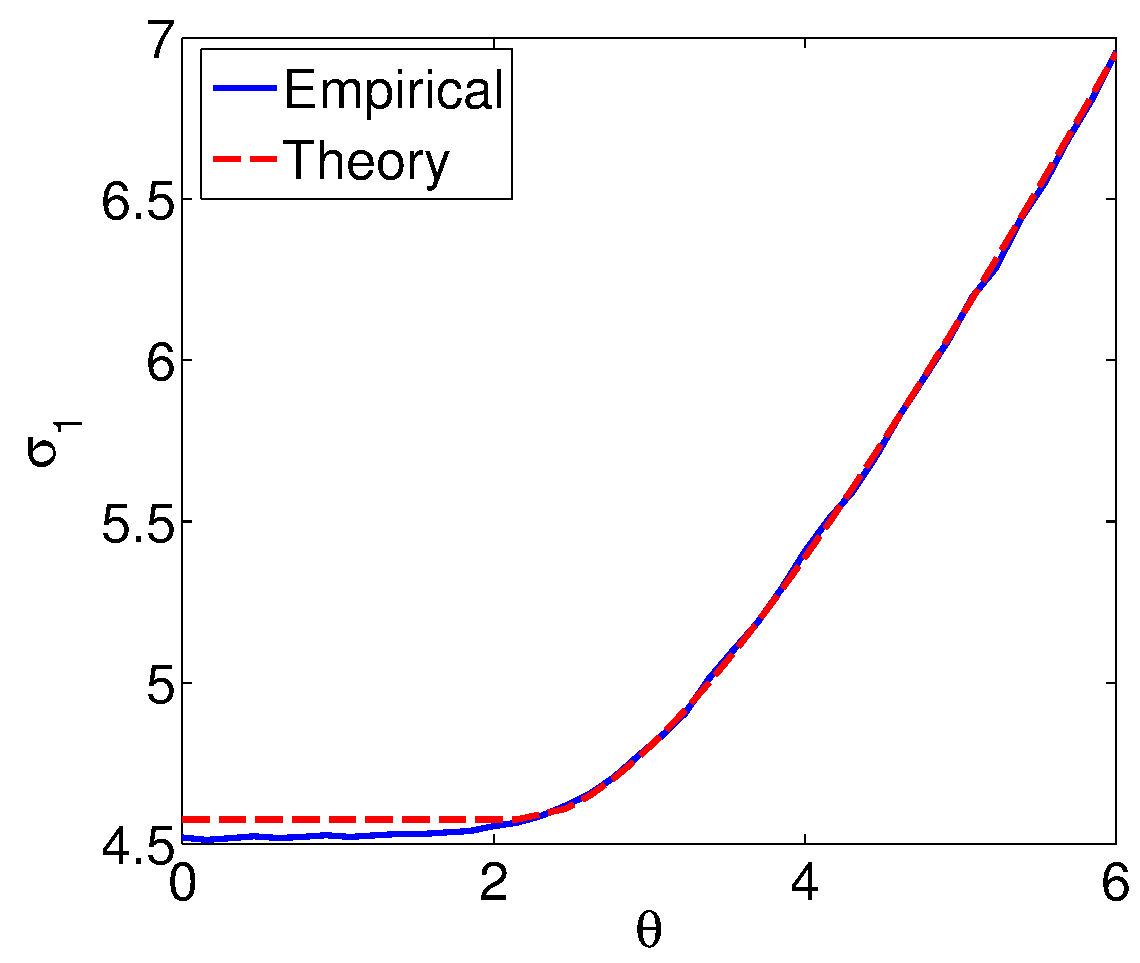
\includegraphics[width=0.47\textwidth]{chpt7_svd_proj/figs/gauss_sv_pred.pdf}
    }
    \subfigure[Gaussian-like $G$]{
      \label{fig:chpt7:gauss_like_pred}
      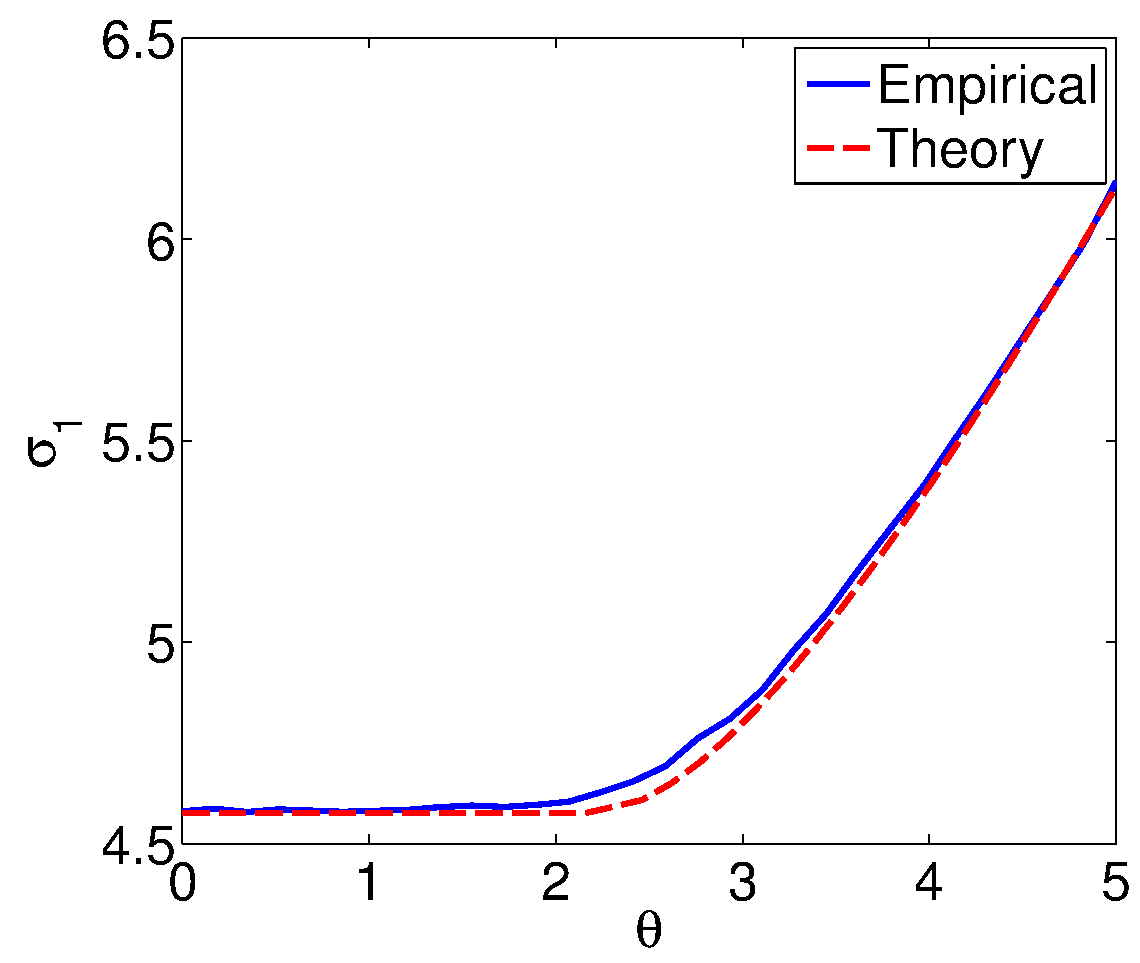
\includegraphics[width=0.47\textwidth]{chpt7_svd_proj/figs/gauss_sweep.pdf}
    }
    \caption{(a) Singular value prediction for Gaussian $G$ and $X$ for a rank-1 setting
      with fixed $n=1000$, $N=1220$ and $m=100$. The theoretical prediction uses
      (\ref{eq:chpt7:solution}) with approximations from Figure
      \ref{fig:chpt7:g_code}. Empirical results are averaged over 500 trials. (b) Singular
      value prediction for Gaussian-like $G$ and Gaussian $X$ for a rank-1 setting with
      fixed $n=1000$, $N=1220$ and $m=100$. Here, the entries of $G$ are either
      $\pm 1$ with equal probability. The theoretical prediction is the same for
      (a). Empirical results are again averaged over 500 trials.}
    \label{fig:chpt7:gauss_sv}
  \end{center}
\end{figure}

We then explore the accuracy of the phase transition boundary for the Gaussian setting in
Figure \ref{fig:chpt7:gauss}. In the first row of this Figure, we plot the KS-statistic
between the largest singular values from these 500 signal and noise only matrices. In the
second row we plot the average top singular value of the signal matrix. All figures set
$n=1000$. The left column sweeps over $\theta$ and $N$ while the right column sweeps over
$\theta$ and $m$. In all figures, we plot our theoretical phase transition prediction in
solid white line. Using a dashed white line, we plot the theoretical phase transition when
no projection is used; this is $\theta=\left(\frac{n}{N}\right)^{1/4}$.

From this figure, we observe that the phase transition prediction is very
accurate. Similarly we notice that the phase transition when using the Gaussian projection
is significantly worse that that when not projecting. The figures in the left column set
$m=100$ so that we reduce our SVD dimension by one order of magnitude. Interestingly, and
perhaps most importantly, when using a Gaussian projection matrix, setting $m=n=1000$
results in worse performance than the non-projecting case even though we aren't reducing
the dimension of the problem. This is evident in the right column.


\begin{figure}
\begin{center}
  \subfigure[KS Statistic - $N$,$\theta$ sweep]{
    \label{fig:chpt7:gauss1}
    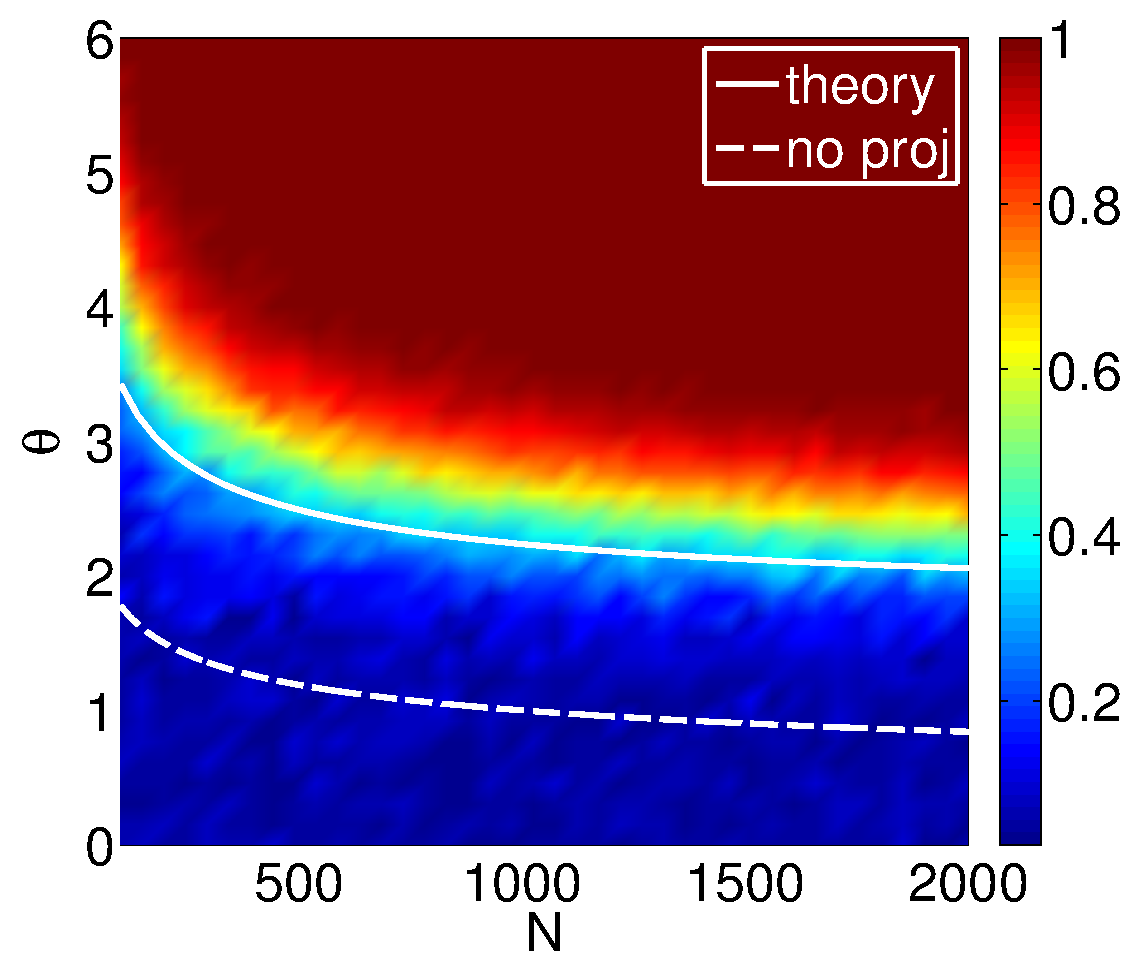
\includegraphics[width=0.47\textwidth]{chpt7_svd_proj/figs/ks11.pdf}
  }
  \subfigure[KS Statistic - $m$,$\theta$ sweep]{
    \label{fig:chpt7:gauss2}
    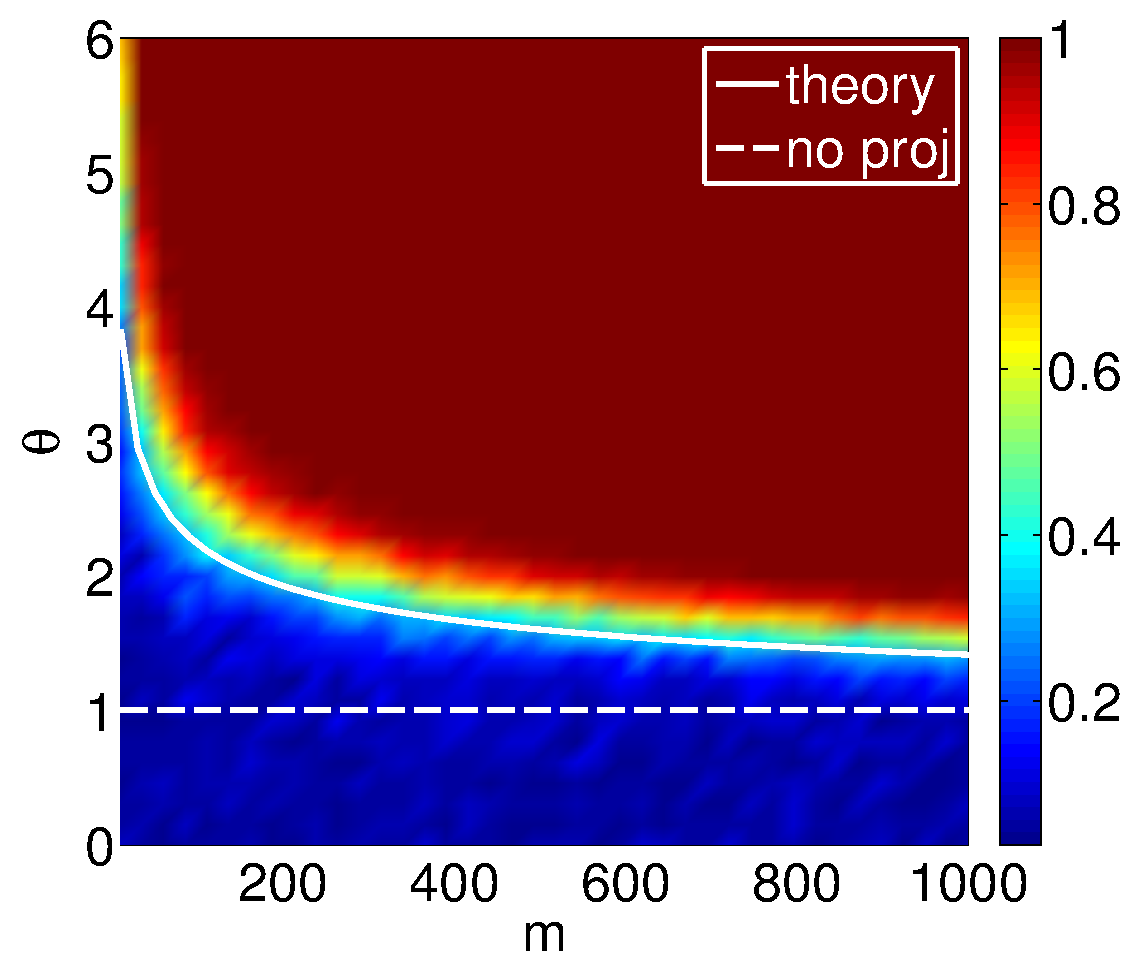
\includegraphics[width=0.47\textwidth]{chpt7_svd_proj/figs/ks21.pdf}
  }
  \subfigure[Maximum singular value - $N$,$\theta$ sweep]{
    \label{fig:chpt7:gauss3}
   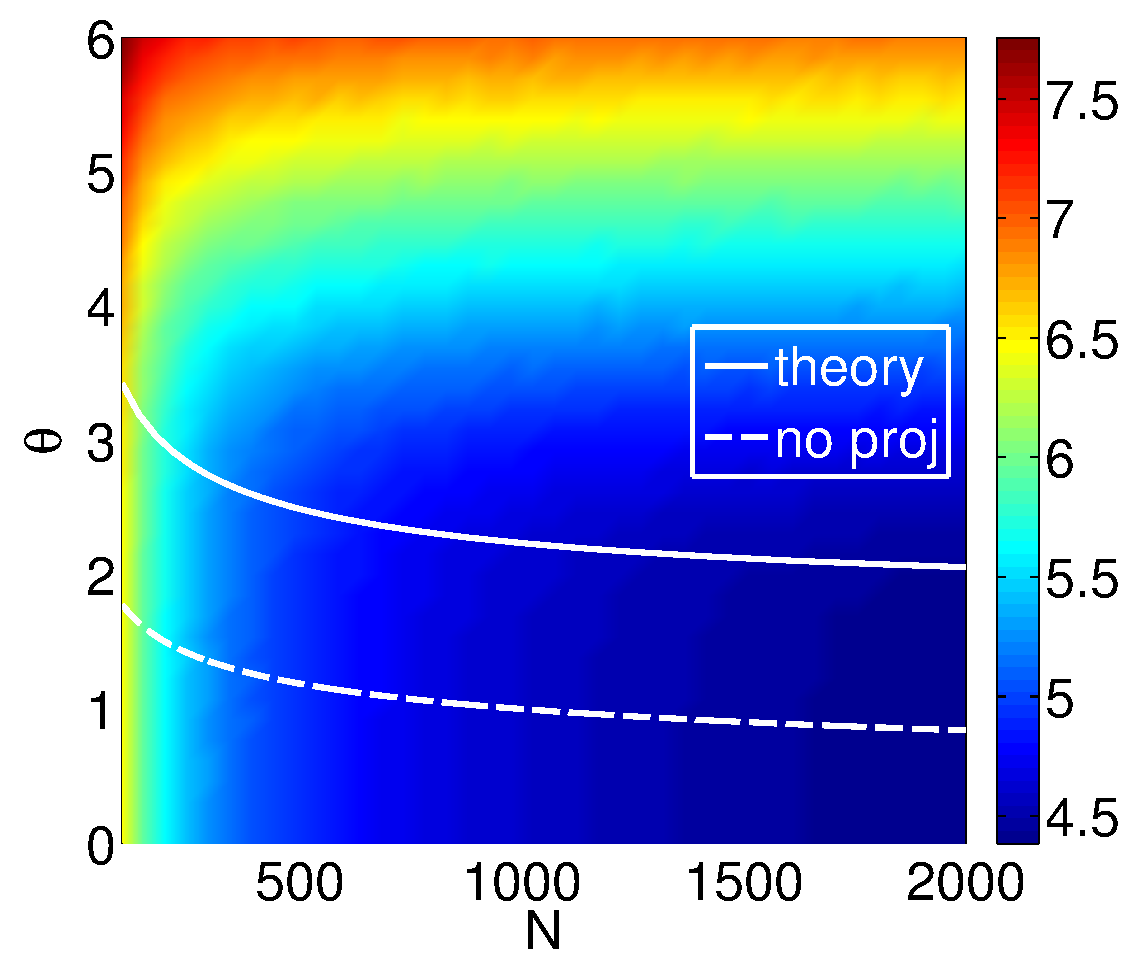
\includegraphics[width=0.47\textwidth]{chpt7_svd_proj/figs/maxsv11.pdf}
  }
  \subfigure[Maximum singular value - $m$, $\theta$ sweep]{
    \label{fig:chpt7:gauss4}
    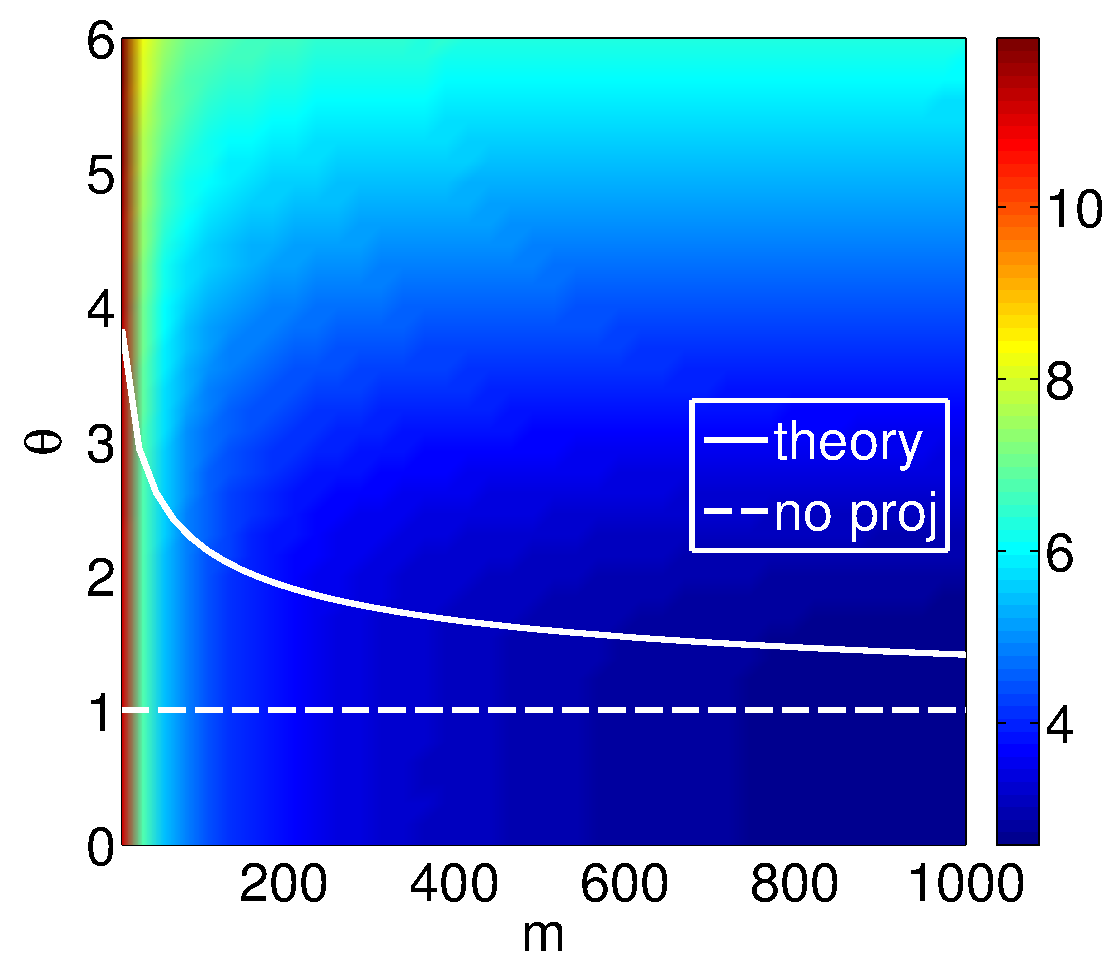
\includegraphics[width=0.47\textwidth]{chpt7_svd_proj/figs/maxsv21.pdf}
  }
%  \subfigure[Singular Vector accuracy $N$,$\theta$ sweep]{
%    \label{fig:chpt7:gauss5}
%   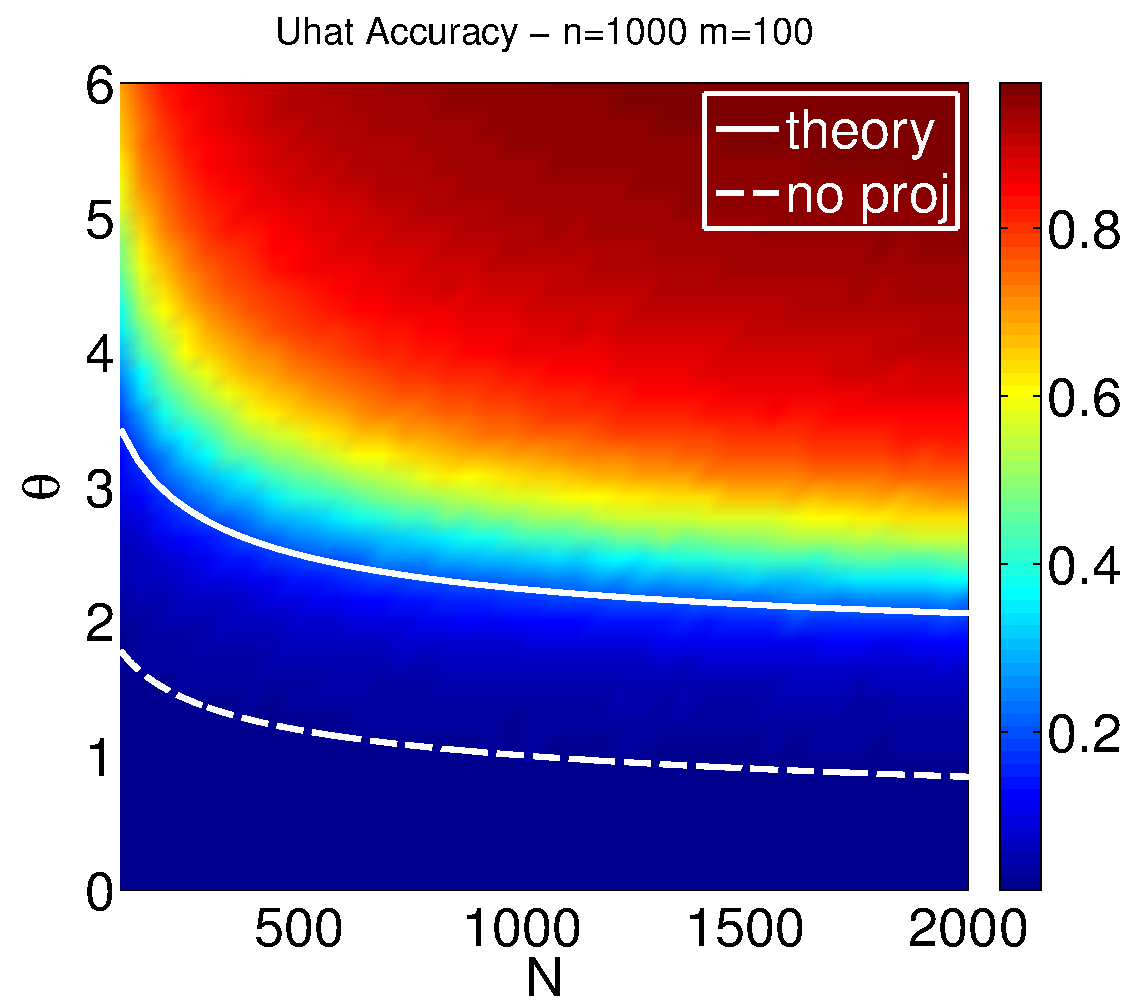
\includegraphics[width=0.47\textwidth]{chpt7_svd_proj/figs/uhat11.pdf}
%  }
%  \subfigure[Singular Vector accuracy $m$,$\theta$ sweep]{
%    \label{fig:chpt7:gauss6}
%    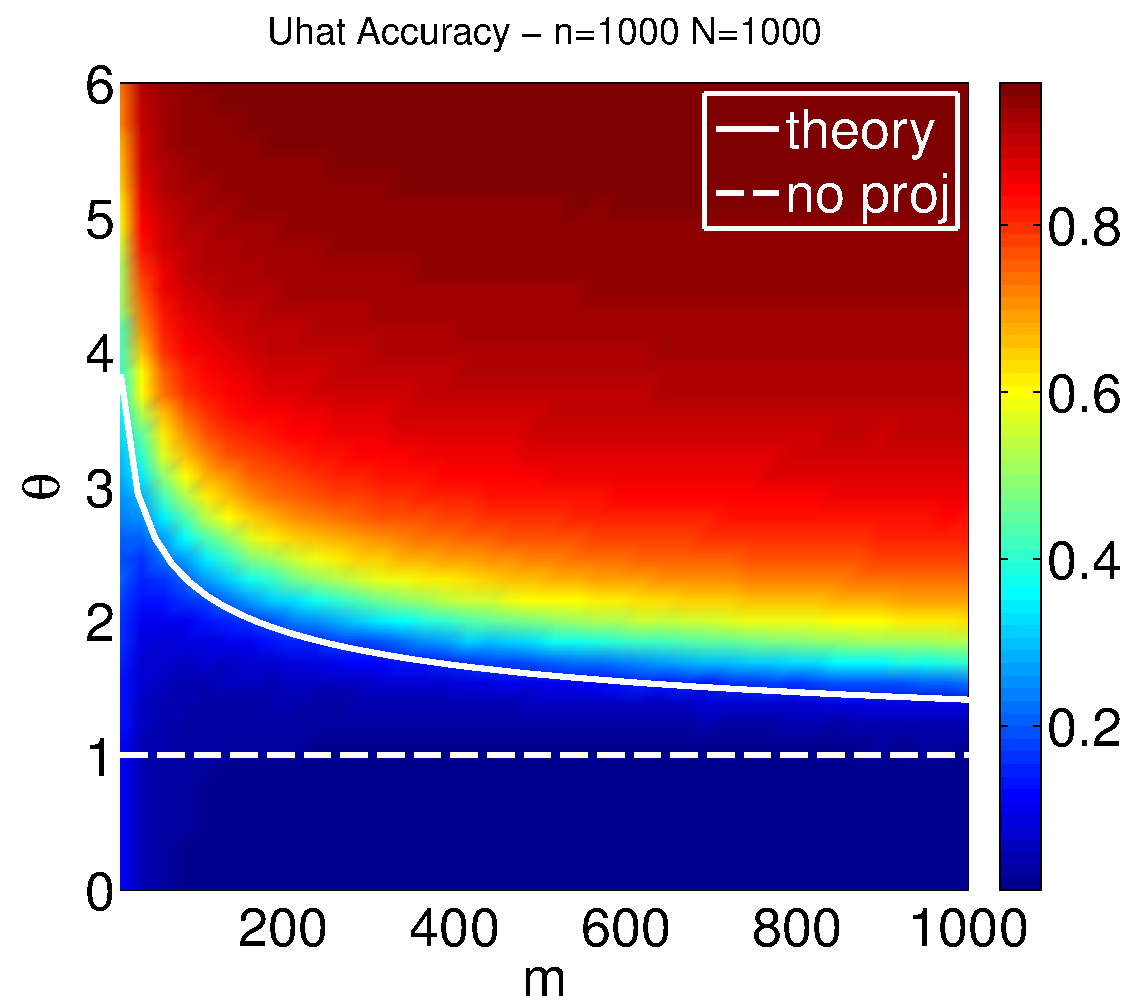
\includegraphics[width=0.47\textwidth]{chpt7_svd_proj/figs/uhat21.pdf}
%  }
  \caption{Performance of theoretical phase transition prediction for Gaussian $G$ and $X$
    for a rank-1 setting with fixed $n=1000$. The theoretical prediction uses
    (\ref{eq:chpt7:solution}) with approximations from Figure \ref{fig:chpt7:g_code}. The
    first row plots the KS statistic between singular values generated from 500 signal
    bearing and 500 noise only matrices. The bottom row plots the average empirical
    singular value averaged over 500 trials. The left column sweeps over both $\theta$ and
    $N$ for a fixed $m=100$ while the right column sweeps over $\theta$ and $m$ for a
    fixed $N=1000$.}
  \label{fig:chpt7:gauss}
\end{center}
\end{figure}

\subsection{Unitary Projection, $Q$}

In this setting, we a unitary projection matrix $Q$ using a QR decomposition of a random
matrix. In {\sc{matlab}} this is accomplished with 
\be 
\texttt{[Q,\textasciitilde] = qr(randn(n)); Q=Q(:,1:m)}.
\ee

Figure \ref{fig:chpt7:ortho_pred} plots the performance of our theoretical prediction when
using a unitary projection matrix, $Q$, for a rank-1 seeting with a fixed $n=1000$,
$N=1220$, $m=100$. In our empirical setup, we generate 500 matrices from
(\ref{eq:chpt7:data_model}) and 500 noise only matrices. We then generate a random $Q$
selected as above. The figure plots the empirical and theoretically predicted top singular
value for a number of $\theta_1=\theta$. The theoretical prediction uses the result from
Corollary \ref{corr:svd_proj_unitary} and does an excellent job at the singular value
prediction. 

In Figure \ref{fig:chpt7:fourier_pred}, we consider a specific choice of unitary
matrix. Here, we randomly select columns from the $n\times n$ discrete Fourier matrix $F$
with entries  
\beq\label{eq:chpt7:fourier}
F_{kj} = \frac{1}{\sqrt{n}}\exp\left\{\frac{-2\pi i (k-1)(j-1)}{n}\right\}
\eeq
for $k=1\dots,n$ and $j=1,\dots,n$. To generate $Q$ we then select $m$ columns from
$F$. We see that the theoretical prediction from Corollary \ref{corr:svd_proj_unitary}
still does an excellent job at the singular value prediction for this specific choice of
unitary matrix. 

\begin{figure}
  \begin{center}
    \subfigure[Unitary $Q$]{
      \label{fig:chpt7:ortho_pred}
      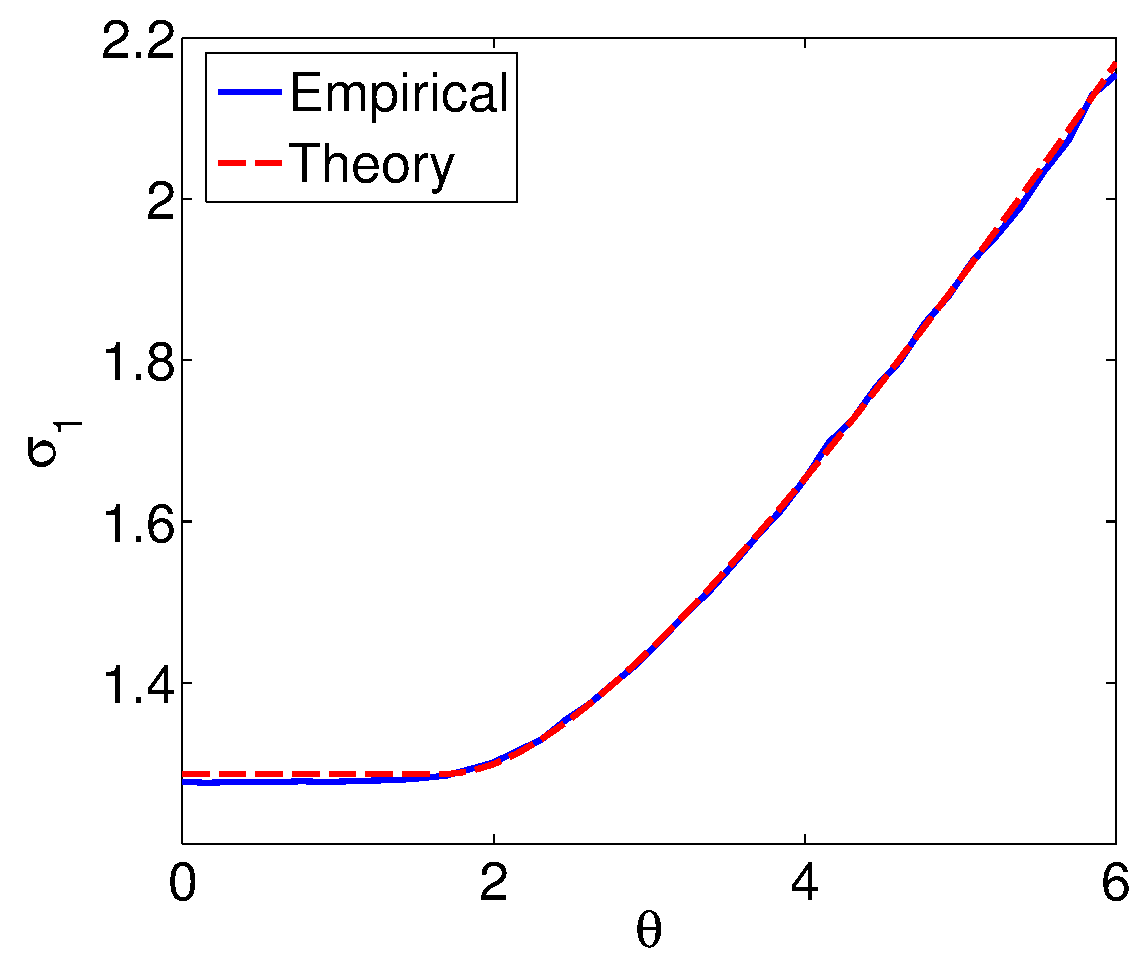
\includegraphics[width=0.47\textwidth]{chpt7_svd_proj/figs/unitary_sv_pred.pdf}
    }
    \subfigure[Fourier $Q$]{
      \label{fig:chpt7:fourier_pred}
      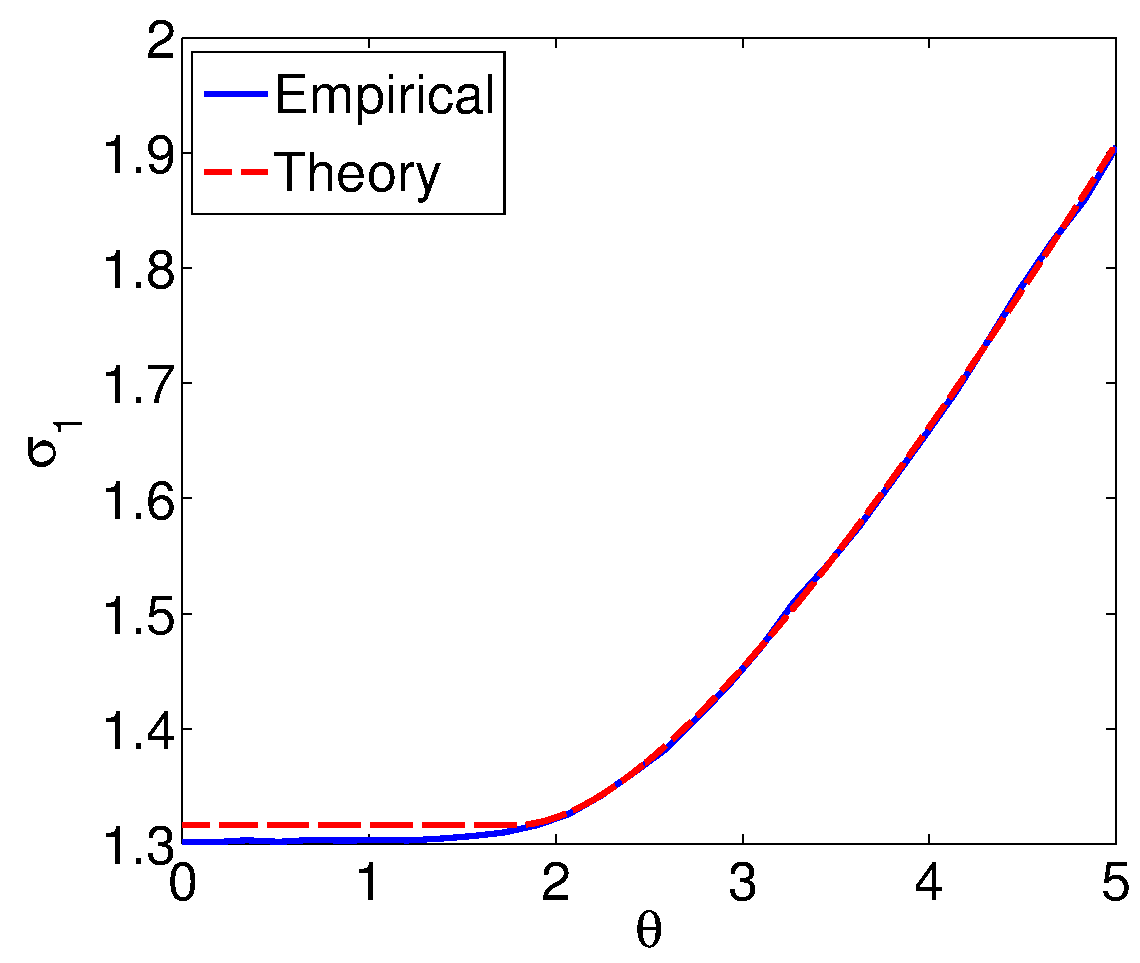
\includegraphics[width=0.47\textwidth]{chpt7_svd_proj/figs/fourier_sweep.pdf}
    }
    \caption{(a) Singular value prediction for unitary projection matrix $Q$ and Gaussian
      noise matrix $X$ for a rank-1 setting with fixed $n=1000$, $N=1220$ and $m=100$. The
      theoretical prediction uses Corollary \ref{corr:svd_proj_unitary}. Empirical results
      are averaged over 500 trials. (b) Singular value prediction for unitary-like matrix
      $Q$ and Gaussian noise matrix $X$ for a rank-1 setting with fixed $n=1000$, $N=1220$
      and $m=100$. Here, the columns of $Q$ are sampled from the $n\times n$ discrete
      Fourier matrix defined in (\ref{eq:chpt7:fourier}). The theoretical prediction is
      the same as (a) and uses Corollary \ref{corr:svd_proj_unitary}. Empirical results
      are averaged over 500 trials.}
    \label{fig:chpt7:ortho_sv}
  \end{center}
\end{figure}

Figure \ref{fig:chpt7:orth_g} plots the performance of our theoretical prediction when
using a unitary projection matrix, $Q$. Our parameter sweep is the same as described for
Figure \ref{fig:chpt7:gauss}, except that here we use the phase transition prediction
given in Corollary \ref{corr:svd_proj_unitary}. Again, we notice that our phase transition
prediction is very accurate. A key observation is that for a unitary projection matrix, as
$m\to n$, the phase transition approaches that of not using a projection matrix. This is
very desirable as we don't want to suffer much performance loss for only slightly reducing
the dimension of the problem.

\begin{figure}
\begin{center}
  \subfigure[KS Statistic - $N$,$\theta$ sweep]{
    \label{fig:chpt7:ortho1}
    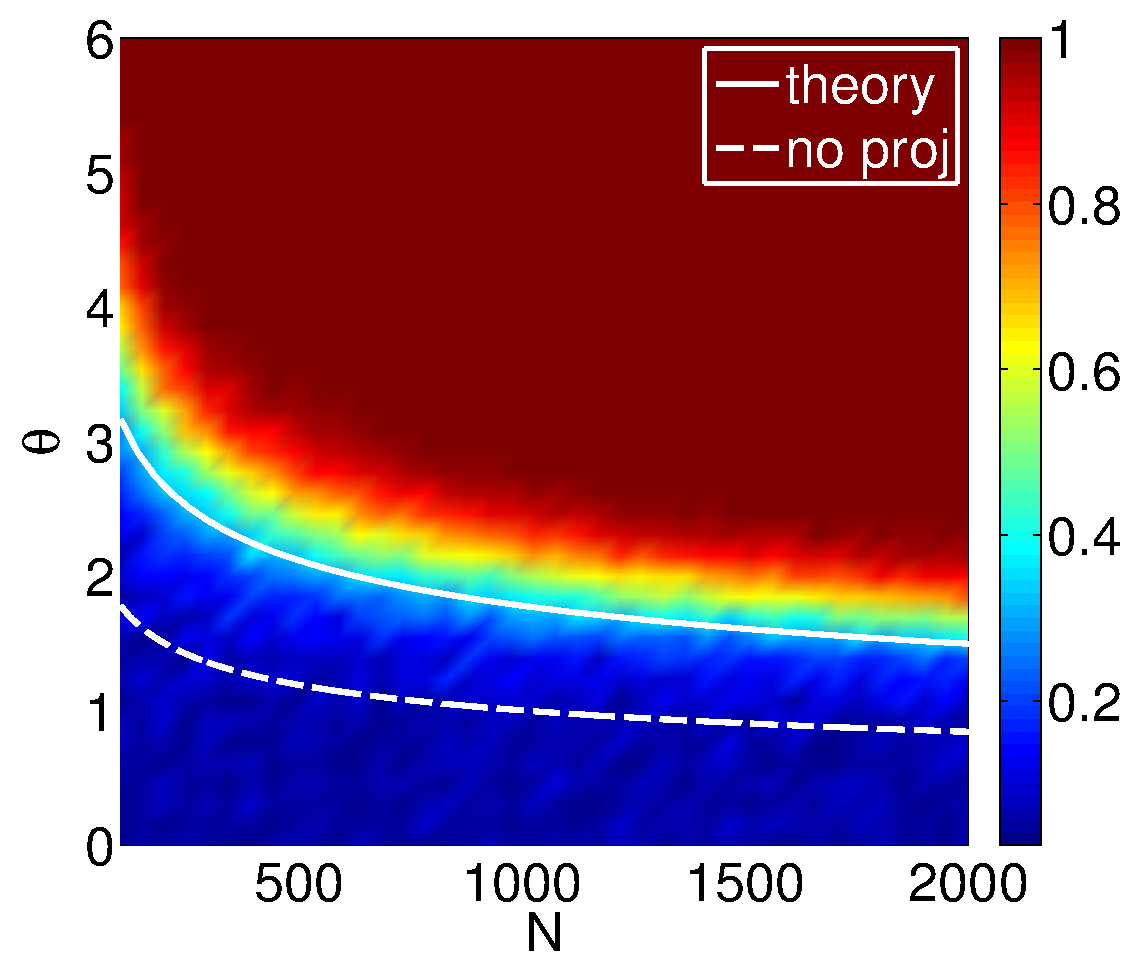
\includegraphics[width=0.47\textwidth]{chpt7_svd_proj/figs/ks12.pdf}
  }
  \subfigure[KS Statistic - $m$,$\theta$ sweep]{
    \label{fig:chpt7:ortho2}
    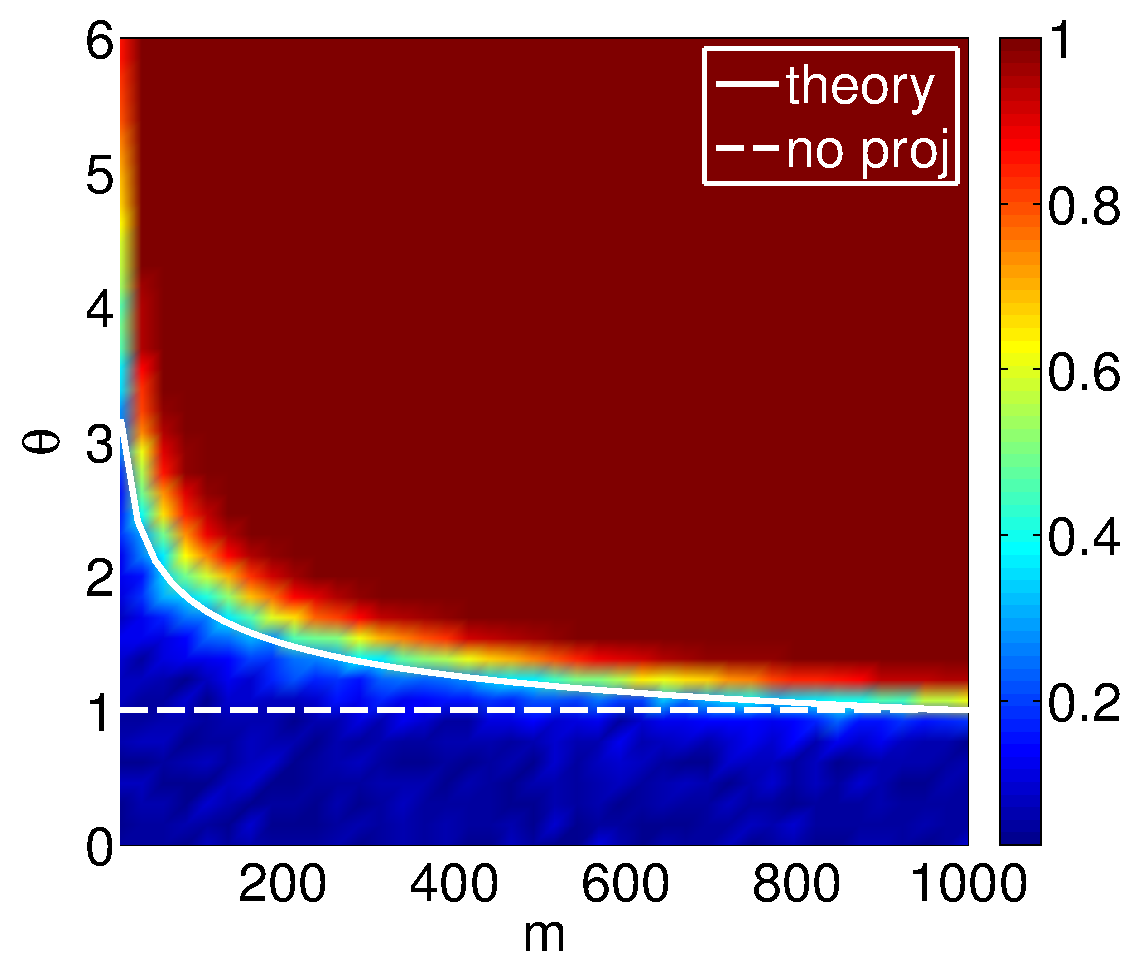
\includegraphics[width=0.47\textwidth]{chpt7_svd_proj/figs/ks22.pdf}
  }
  \subfigure[Maximum singular value - $N$,$\theta$ sweep]{
    \label{fig:chpt7:ortho3}
   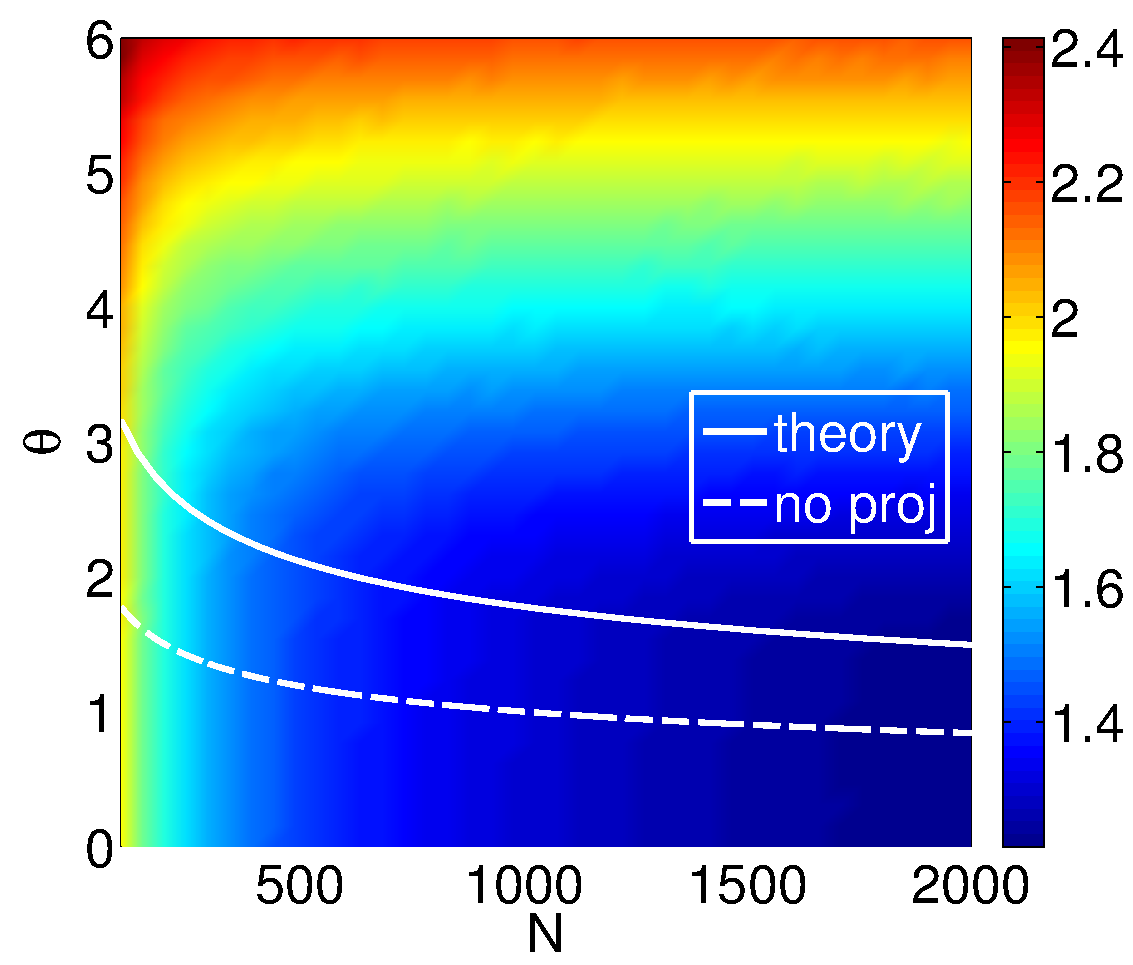
\includegraphics[width=0.47\textwidth]{chpt7_svd_proj/figs/maxsv12.pdf}
  }
  \subfigure[Maximum singular value - $m$, $\theta$ sweep]{
    \label{fig:chpt7:ortho4}
    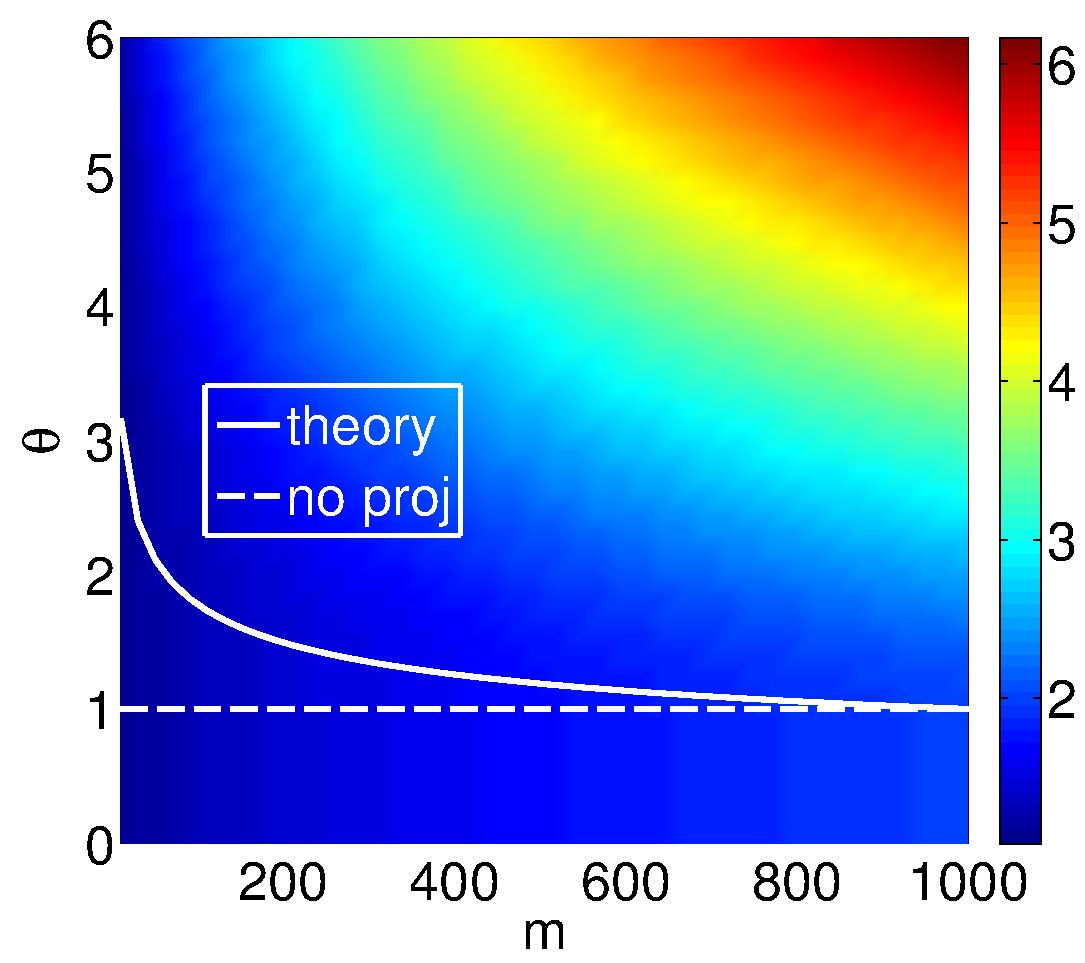
\includegraphics[width=0.47\textwidth]{chpt7_svd_proj/figs/maxsv22.pdf}
  }
%  \subfigure[Singular Vector accuracy $N$,$\theta$ sweep]{
%    \label{fig:chpt7:ortho5}
%   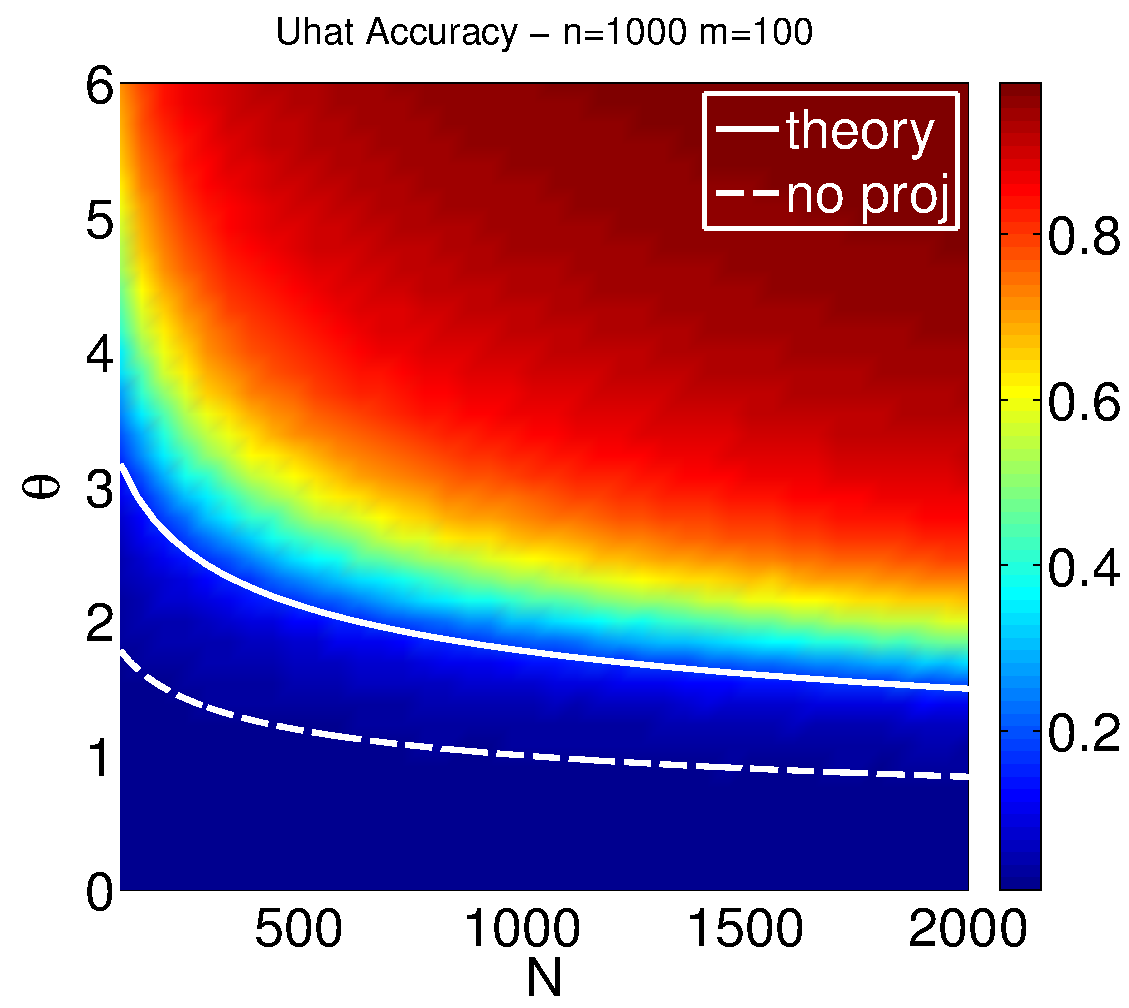
\includegraphics[width=0.47\textwidth]{chpt7_svd_proj/figs/uhat12.pdf}
%  }
%  \subfigure[Singular Vector accuracy $m$,$\theta$ sweep]{
%    \label{fig:chpt7:ortho6}
%    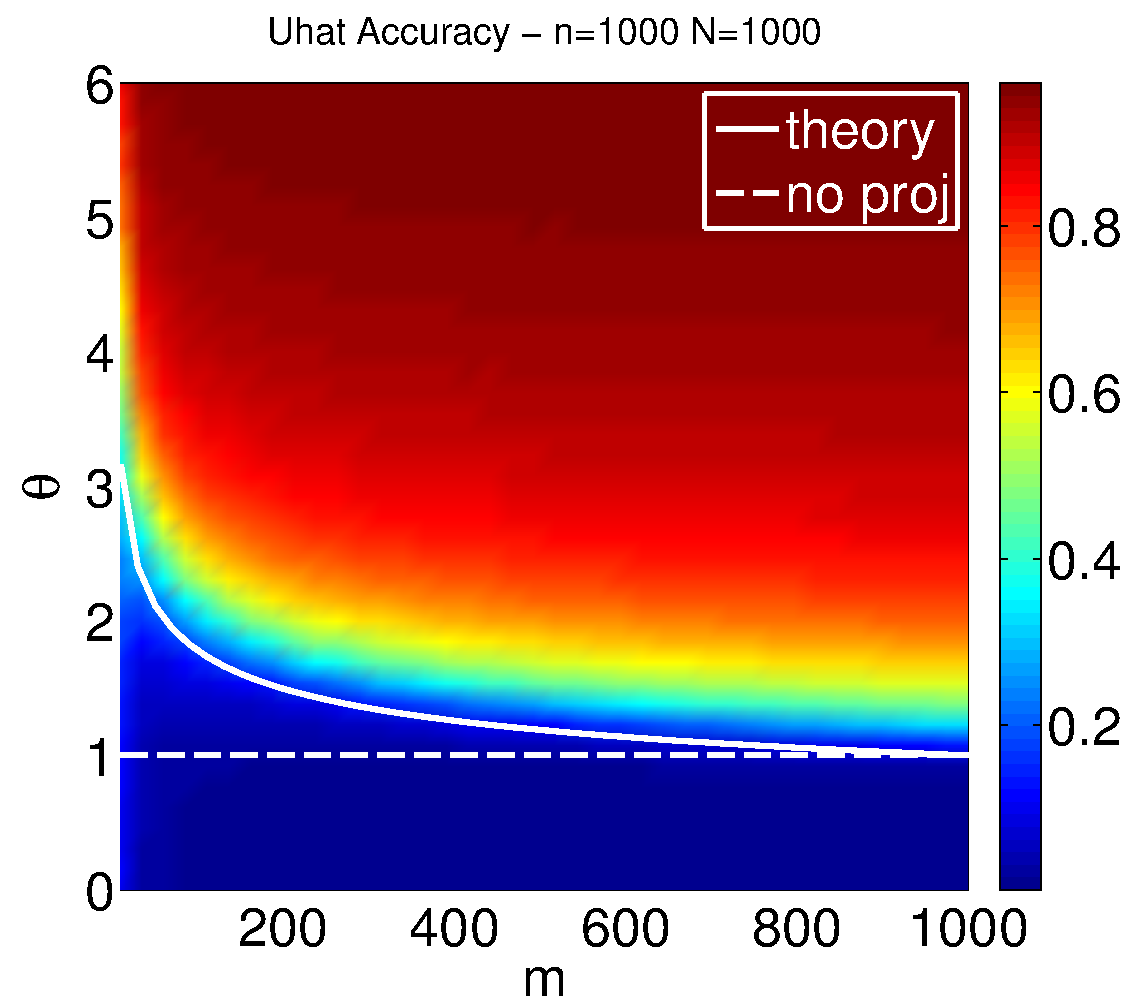
\includegraphics[width=0.47\textwidth]{chpt7_svd_proj/figs/uhat22.pdf}
%  }
  \caption{Performance of theoretical phase transition prediction for unitary projection
    matrix $Q$ and Gaussian noise matrix $X$ for a rank-1 setting with fixed $n=1000$. The
    theoretical prediction uses Corollary \ref{corr:svd_proj_unitary}. The first row plots
    the KS statistic between singular values generated from 500 signal bearing and 500
    noise only matrices. The bottom row plots the average empirical singular value
    averaged over 500 trials. The left column sweeps over both $\theta$ and $N$ for a
    fixed $m=100$ while the right column sweeps over $\theta$ and $m$ for a fixed
    $N=1000$.}
  \label{fig:chpt7:orth_g}
\end{center}
\end{figure}

\subsection{Comparison}

Here we discuss the difference between the two choices of projection matrices. Figure
\ref{fig:chpt7:comparison} shows the empirical difference of the KS statistic plots from
Figures \ref{fig:chpt7:gauss} and \ref{fig:chpt7:orth_g}. On each plot we overlay the
theoretical phase transition lines. The solid white is the prediction for a Gaussian
projection matrix from (\ref{eq:chpt7:solution}) using the method in Figure
\ref{fig:chpt7:g_code}; the dashed white is the prediction for an unitary projection matrix
from Corollary \ref{corr:svd_proj_unitary}; the solid black is the prediction when
not using a projection ($\theta=c^{1/4}$). Positive values in these plots indicate that
the top singular value using a Gaussian projection matrix can more reliably detect our one
signal; negative values indicate that the top singular value using a unitary projection
matrix can more reliably detect our signal. The first column sweeps over $N$ and $\theta$
for a fixed $m=100$ and $n=1000$ while the second column sweeps over $m$ and $\theta$ for
a fixed $N=1000$ and $n=1000$.

We see that the unitary projection matrix performs uniformly better than the Gaussian
projection matrix above the phase transition. Below their respective phase transitions,
all methods fail. Importantly, even when setting $m=n$ so that the projection doesn't
reduce the dimension, the unitary projection keeps the same phase transition while the
Gaussian projection changes the phase transition so that it is harder to detect the
presence of a signal. This allows us to conclude that in terms of detection performance,
the unitary projection matrix is better than the Gaussian projection matrix. 

However, we do note that generating these projection matrices, particularly for large
dimensions, is important. Generating the Gaussian projection matrix $G$ is very easy as
every entry is an independent Gaussian random variable. However, generating a $n\times m$
unitary matrix $Q$ for high dimensions may be prohibitive. The analysis in this chapter
gives the practitioner the ability to choose the projection matrix that best fits his or
her needs. Given system parameters, the practitioner can select the projection dimension
$m$ to achieve a certain detection ability. The decision may be driven by the ease of
creating each projection matrix.

\begin{figure}
\begin{center}
  \subfigure[KS Statistic difference - $N$,$\theta$ sweep]{
    \label{fig:chpt7:comp1}
    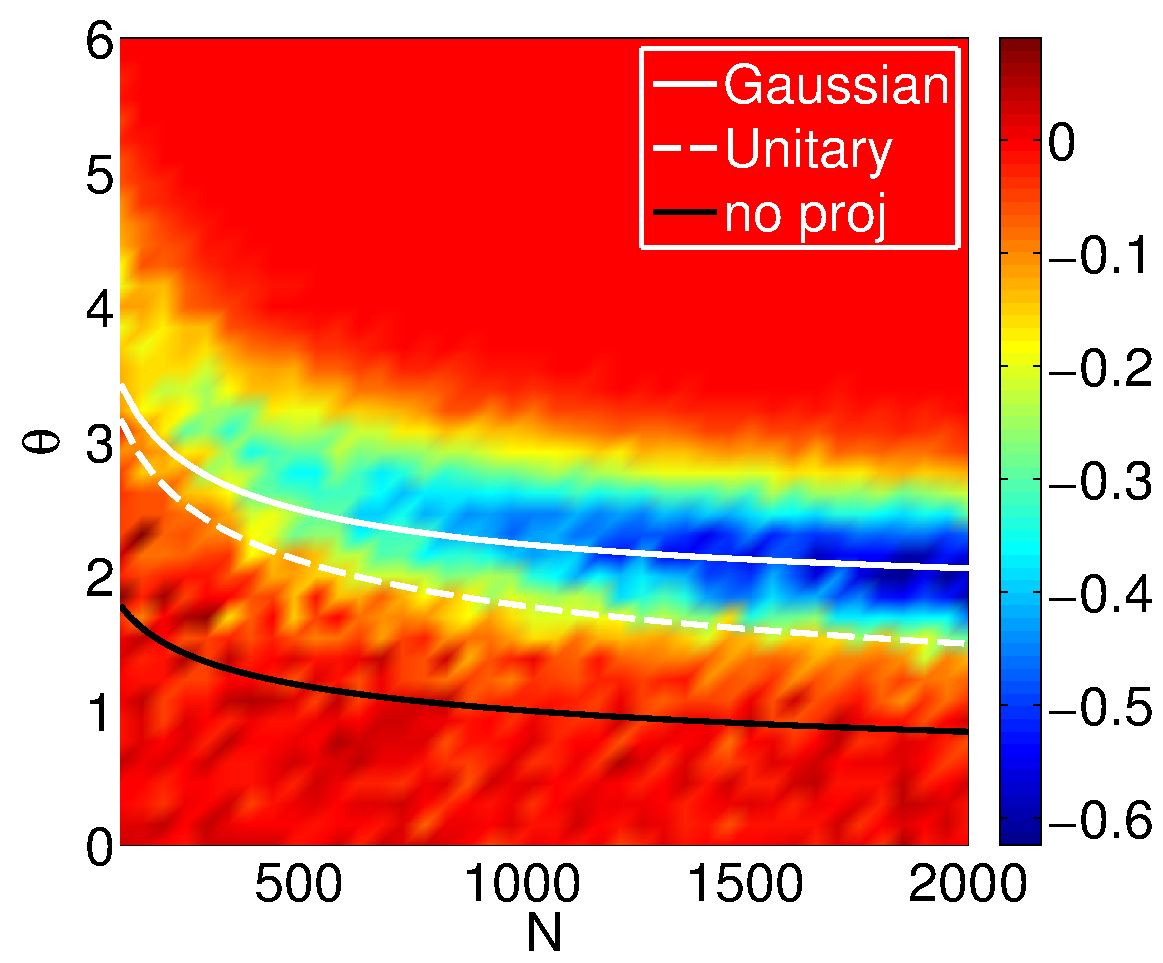
\includegraphics[width=0.47\textwidth]{chpt7_svd_proj/figs/ksdiff1.pdf}
  }
  \subfigure[KS Statistic difference - $m$,$\theta$ sweep]{
    \label{fig:chpt7:comp2}
    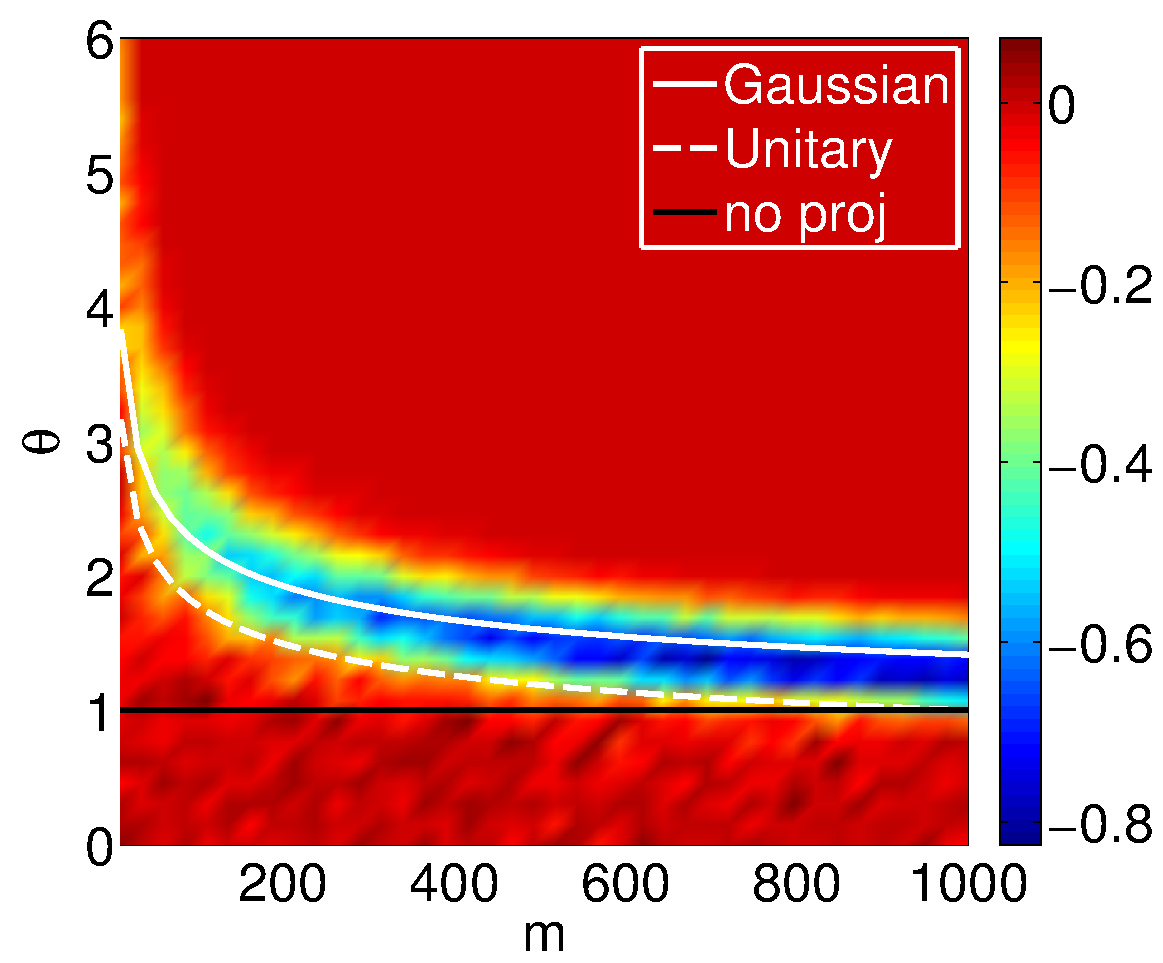
\includegraphics[width=0.47\textwidth]{chpt7_svd_proj/figs/ksdiff2.pdf}
  }
%  \subfigure[Maximum singular value difference - $N$,$\theta$ sweep]{
%    \label{fig:chpt7:comp3}
%   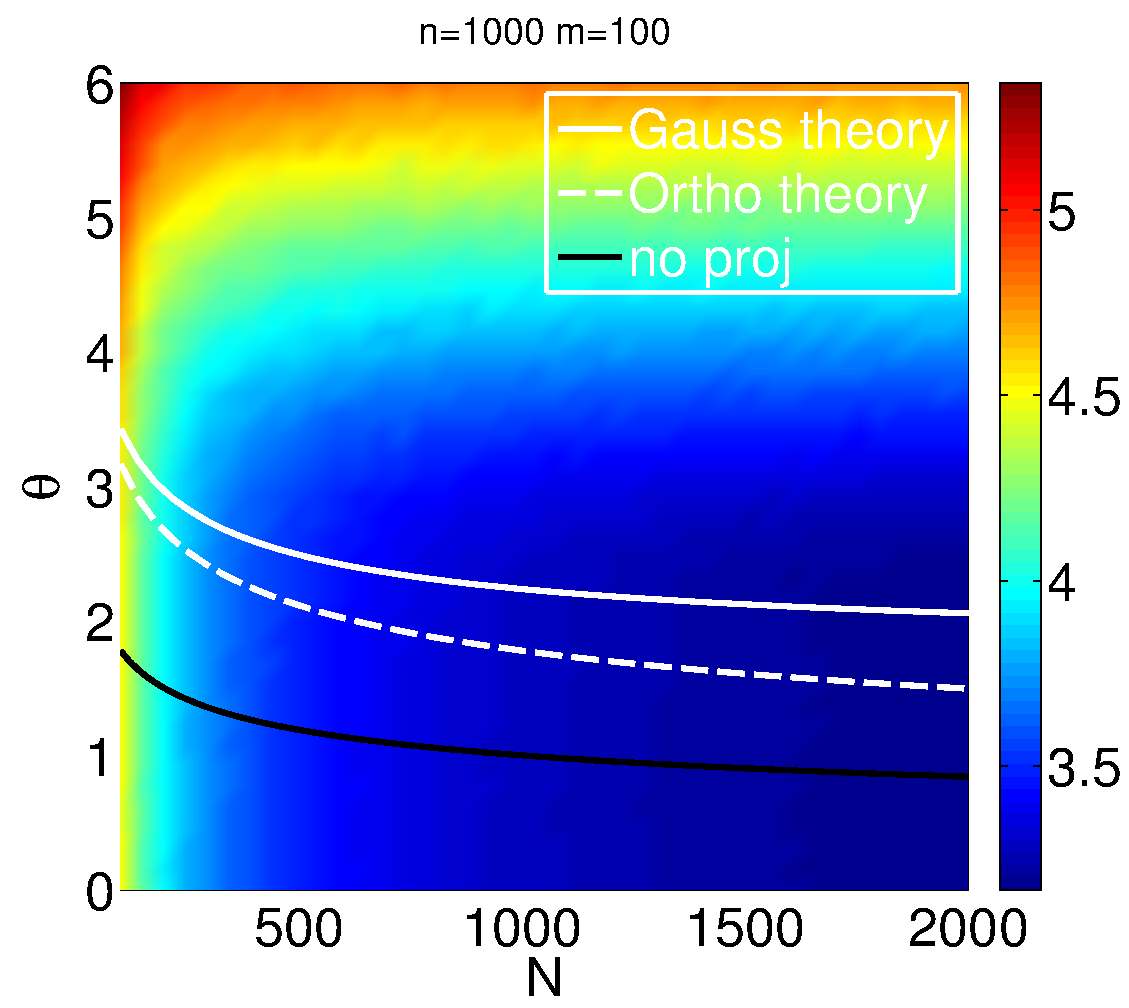
\includegraphics[width=0.47\textwidth]{chpt7_svd_proj/figs/svdiff1.pdf}
%  }
%  \subfigure[Maximum singular value difference - $m$, $\theta$ sweep]{
%    \label{fig:chpt7:comp4}
%    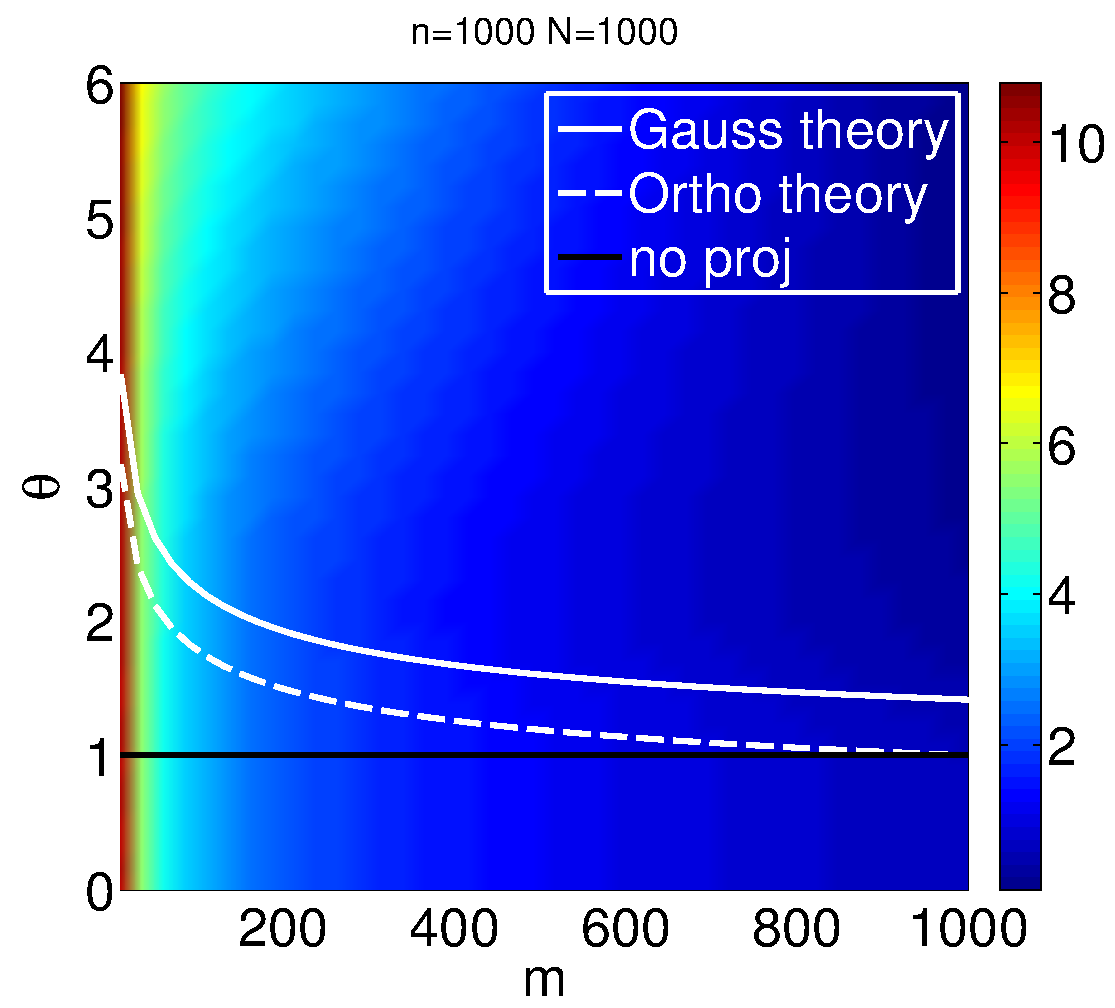
\includegraphics[width=0.47\textwidth]{chpt7_svd_proj/figs/svdiff2.pdf}
%  }
%  \subfigure[Singular Vector accuracy difference $N$,$\theta$ sweep]{
%    \label{fig:chpt7:comp5}
%   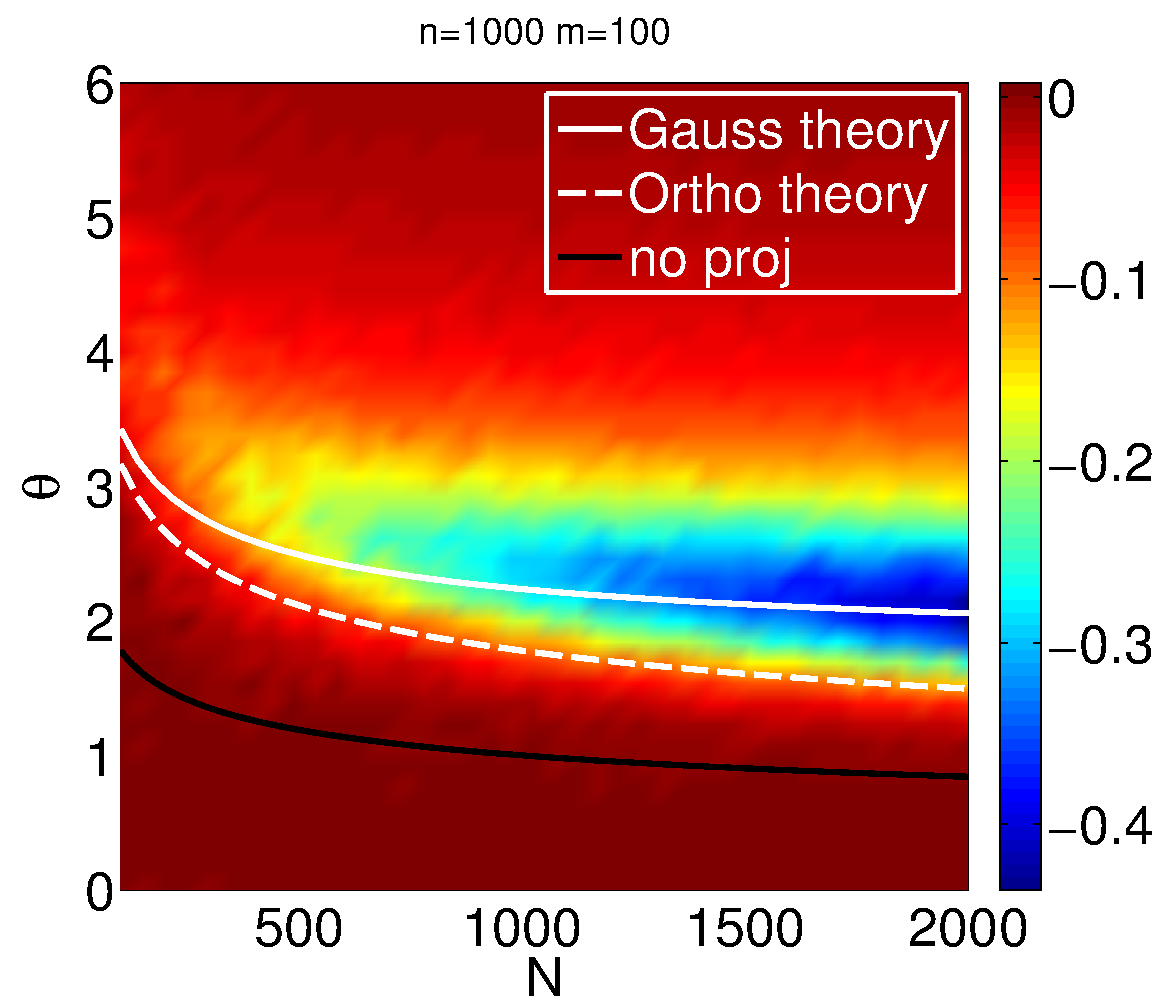
\includegraphics[width=0.47\textwidth]{chpt7_svd_proj/figs/uhatdiff1.pdf}
%  }
%  \subfigure[Singular Vector accuracy difference $m$,$\theta$ sweep]{
%    \label{fig:chpt7:comp6}
%    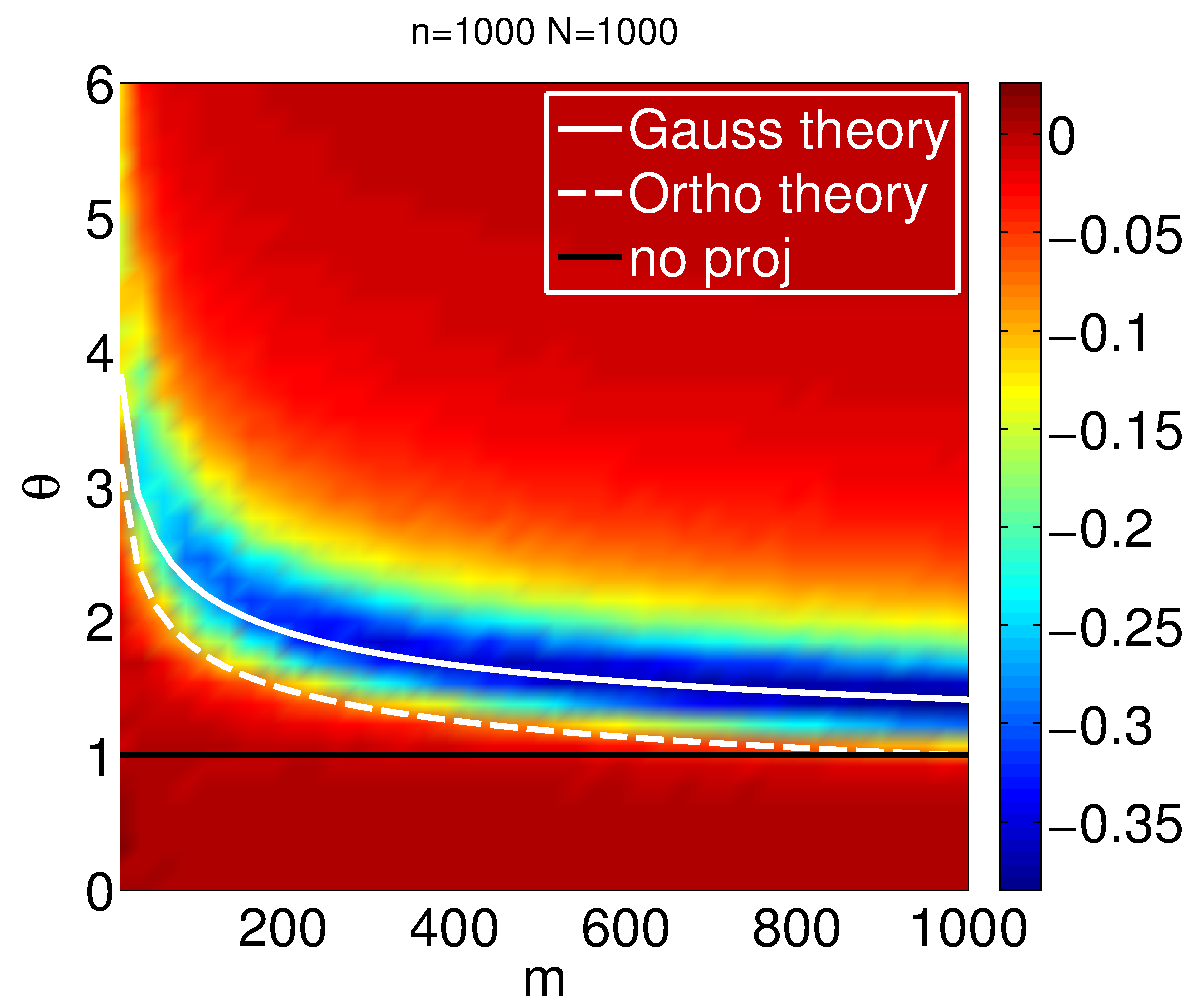
\includegraphics[width=0.47\textwidth]{chpt7_svd_proj/figs/uhatdiff2.pdf}
%  }
  \caption{Performance difference between using a Gaussian projection matrix, $G$, and a
    unitary projection matrix, $Q$, for a rank-1 setting with fixed $n=1000$ and Gaussian
    noise matrix $X$. Positive values indicate that the Gaussian projection can more
    reliably detect the signal while negative values indicate that the unitary projection
    can more reliably detect the signal. We observe that the unitary projection
    outperforms the Gaussian projection.}
  \label{fig:chpt7:comparison}
\end{center}
\end{figure}

